\documentclass[11pt,edeposit,draftthesis]{uiucthesis2020}

% {{{ packages

\usepackage{blindtext}
\usepackage{cite}
\usepackage{array}

% math
\usepackage{fixmath}
\usepackage{amsmath}
\usepackage{amsthm}
\usepackage{amssymb}
\usepackage{stmaryrd}

% pretty links
\usepackage{xparse}
\usepackage{hyperref}
\usepackage{cleveref}
\usepackage{graphicx}
\hypersetup{
    colorlinks=true,
    urlcolor=blue,
    citecolor=black,
    linkcolor=black
}

% better environments
\usepackage[shortlabels]{enumitem}
\usepackage{booktabs}

% fancier font
\usepackage[sc]{mathpazo}
% better typography
\usepackage[activate={true,nocompatibility}, % activate protrusion and font expansion
            final,              % enable microtype, use draft to disable
            tracking=true,
            kerning=true,       % optimise interactions between characters
            spacing=true,       % more uniform spacing between words
            factor=1100,        % more protrusion
            stretch=10,         % smaller values (default 20, 20) to avoid blurring
            shrink=10]{microtype}
\microtypecontext{spacing=nonfrench}
\SetTracking{encoding={*}, shape=sc}{40}

% }}}

% {{{ commands

\NewDocumentCommand \dx { O{x} } {\,\mathrm{d} #1}
\NewDocumentCommand \vect { m } { \mathbold{#1} }
\NewDocumentCommand \jump { m } { \left\llbracket #1 \right\rrbracket }
\NewDocumentCommand \avg { m } { \left\langle #1 \right\rangle}
\NewDocumentCommand \od { m m } { \dfrac{\mathrm{d} #1}{\mathrm{d} #2} }
\NewDocumentCommand \pd { m m } { \dfrac{\partial #1}{\partial #2} }

% }}}

% {{{ title

\title{Magnetic ordering and spin wave dynamics in transition metal arsenides}
\author{Manohar H. Karigerasi}
\department{Materials Science and Engineering}

\schools{
B. Tech., Indian Institute of Technology Roorkee, 2016 \\
M. S., University of Illinois at Urbana-Champaign, 2017
}

\phdthesis
\advisor{Daniel P. Shoemaker}
\degreeyear{2021}

\committee{
Associate Professor Daniel P. Shoemaker, Chair \\
Professor David G. Cahill \\
Professor Jian-Min Zuo \\
Research Assistant Professor Gregory MacDougall \\
}

% }}}

\begin{document}

\maketitle

% {{{ front matter

\begin{frontmatter}

\begin{abstract}
Metallic antiferromagnets have gained interest in recent times due to the possibility of being useful as a memory device. Arsenic forms a large pool of magnetic metals in combination with other transition metals that have largely been ignored so far. In this report, we discover a new ternary metallic arsenide in the Cu-Mn-As phase space, identify its chemical and magnetic structure, and characterize its electrical and magnetic properties. We also carry out the magnetic structure refinement of Mn$_3$As$_2$ from neutron powder diffraction data at different temperatures to understand the magnetic ordering in Mn-As compounds. Using inelastic neutron scattering measurements, we determine exchange interactions in Fe$_2$As, which has the same structure as CuMnAs, showing a highly 2D magnon character although the phonons are 3D. Finally, we report a magnetic-structural coupled transition across 300 K in tetragonal CuMnAs and determine the correct magnetic structure of the compound.
\end{abstract}

\chapter*{Acknowledgments}

This project would not be possible without many people. Firstly, thanks to my advisor, Prof. Daniel P. Shoemaker.

%\begin{dedication}
%To Coffee
%\end{dedication}

\tableofcontents
\listoftables
\listoffigures

\end{frontmatter}

% }}}

% {{{ main matter

\begin{mainmatter}

%##################chapter 1
\chapter{Introduction}

\section{Magnetic information storage}

% Information 
In information memory storage devices, there is typically a trade-off between the optimum speed or response time and the complexity and size of memory storage \cite{Wing1986}. Volatile memory refers to temporary memory storage where the data is lost when the power is removed. Volatile memory such as SRAM (static random access memory) and DRAM (dynamic random access memory) are used as CPU caches and main memory respectively. SRAM has much faster access times and does not require periodic refreshing. However, it requires four to six transistors per bit as compared to one transistor and one capacitor in DRAM devices \cite{Meena2014}. Non-volatile memory (NVM) storage devices on the other hand, retain their data for a long period of time until perturbed. Modern computers mostly use flash memory based solid state drives (SSD) and magnetic hard disk drives (HDD) for storing large amounts of data permanently \cite{Meena2014}. The first HDD was invented in 1956 by IBM and since then, has seen more than eight orders of magnitude improvement in the storage density. However, the trilemma in magnetic recording between poor thermal stability, coercive fields and signal-to-noise ratio has resulted in the HDD reaching a saturation limit in their device performance \cite{Krishnan2016}. Flash memory uses floating gate MOSFETs (metal oxide semiconductor field effect transistors) to store memory and does not contain any moving parts. Although SSD have dominated the NVM marketshare last few years, there is an increasing need for alternative NVM technologies that are fast, low power consuming and have high storage density \cite{Meena2014}.

% Emerging NVM
One such emerging NVM is MRAM (magnetoresistive random access memory). Unlike flash memory which uses electronic charge as a medium of memory storage, MRAM uses the electronic spin degree of freedom to store information. Unlike charge based storage devices, MRAM is stable against perturbations such as ionizing radiation \cite{Wadley2016}. MRAM devices consist of cells with magnetic tunnel junctions (MTJ) that have two ferromagnet (FM) layers separated by an insulating layer. One of the layer is pinned where the magnetization orientation is fixed and acts as a reference layer. Depending on the orientation of the free layer, the tunneling magnetoresistance (TMR) is high or low and hence, memory can be read out using electrical currents \cite{Krishnan2016}. Early MRAMs were written by induced fields from heavy currents passed on the adjacent layer. With recent developments in spin transfer torque (STT) in ferromagnets, it has become possible to write using electrical currents \cite{Chappert2007}. This has reduced the power consumption significantly and made commercialization of MRAM devices possible \cite{Krishnan2016,Bhatti2017}.

\section{Antiferromagnets for potential applications as a memory unit}

% Gomonay 2010 paper
Historically, antiferromagnets (AFM) have been used as inactive components in MTJ, primarily in exchange biasing the pinned FM layer. However in 2010, Gomonay \emph{et al.} \cite{Gomonay2010} proposed electrical switching of AFMs using STT by passing a spin polarized current injected from a fixed FM layer through the AFM layer. The electrical current gets spin polarized in the FM layer and transfers its angular momentum to the AFM moments to switch it from one orientation to another. There are advantages to using AFM over FM in MRAM devices. AFM are not easily affected by external magnetic fields and do not produce stray fields of their own. They have smaller domains which would allow for higher storage densities \cite{Wadley2016}. Since the precession frequency of AFM moments is determined the geometric mean of exchange and anisotropy energies, the dynamics in AFM materials occur at THz timescales which is two orders of magnitude higher than in FM \cite{Siddiqui2020}. Although the AFM can be switched using electrical currents from parallel to perpendicular orientation with respect to the FM magnetization direction, the reverse process cannot be obtained using electrical current. High magnetic fields above the spin flop transition of the AFM needs to be applied in order to switch back the AFM to its original state \cite{Gomonay2010}.

% Wadley 2016 paper
Unlike previously discussed STT MRAM devices, spin orbit torque based electrical switching in broken inversion symmetry FM does not require the presence of a FM polarizer \cite{Manchon2008}. This concept of the presence of relativistic fields is applicable to AFM as well provided the local moments do not sit on centrosymmetric sites. If the two sublattices are related to each other by a center of inversion, then the current induced spin polarized fields are staggered across the two sublattices \cite{Zelezny2014,Zelezny2017,Wadley2016}. This results in a uniform fieldlike torque experienced by the order parameter. This is possible in bulk materials that are globally centrosymmetric but locally non-centrosymmetric and the two sublattices are related to each other by a center of inversion. It was initially demonstrated in the case of epitaxially grown tetragonal CuMnAs thin films on GaP substrate \cite{Wadley2016} and since then, it has also been shown in Mn$_2$Au and CuMnAs sputtered films as well \cite{Meinert2018,Matalla-Wagner2019}. Observation of electrical switching behavior in AFM requires the presence of degenrate N\'eel vectors like in CuMnAs as shown in Fig. \ref{fig:tet-CuMnAs}(a) as opposed to compounds like MnF$_2$ where the Mn moments point along $c$ in Fig. \ref{fig:tet-CuMnAs}(b).


\begin{figure}
\centering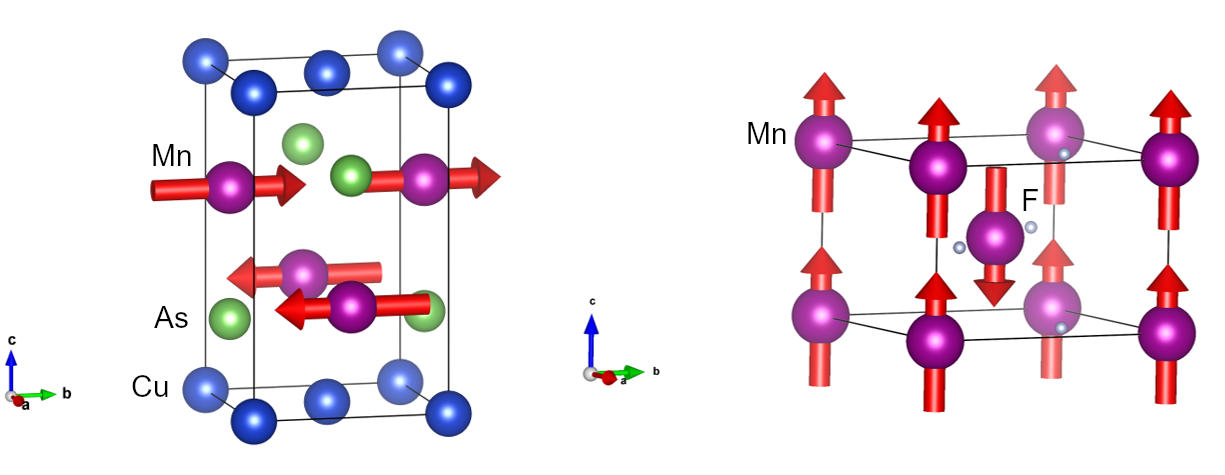
\includegraphics[width=\columnwidth]{figures/ch1/CuMnAs-MnF2.png} \\
\caption{\label{fig:tet-CuMnAs}
The magnetic structures of tetragonal CuMnAs and MnF$_2$ are shown in (a) and (b), respectively.
}
\end{figure}

\section{Exploration of Cu-Mn-As phase space}

% Why are CuMnAs compounds popular?
Compounds in Cu-Mn-As phase space have attracted a lot of attention in recent times mainly due to the exotic properties of tetragonal and orthorhombic CuMnAs. As mentioned earlier, tetragonal CuMnAs was the first antiferromagnet where electrical switching was supposedly demonstrated. Orthorhombic CuMnAs, shown in Fig. \ref{fig:ort-CuMnAs}, was the first magnetic compound to be proposed as a Dirac semimetal. It is a special compound where the inversion and time reversal symmetry of the magnetic structure is broken but their combined symmetry ($PT$ symmetry) is still preserved. Based on the orientation of the AFM order parameter, the compound changes from a conducting to an insulating phase. Hence, there are voltage based switching applications that have been proposed for this compound \cite{Kim2018}.

\begin{figure}
\centering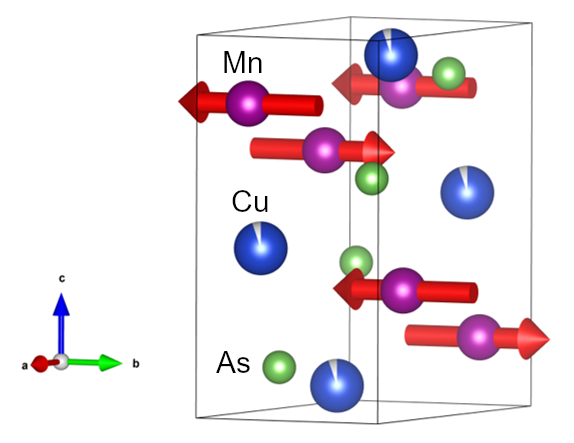
\includegraphics[width=0.5\columnwidth]{figures/ch1/ort-CuMnAs.png} \\
\caption{\label{fig:ort-CuMnAs}
Magnetic structure of orthorhombic CuMnAs
}
\end{figure}


\begin{figure}
\centering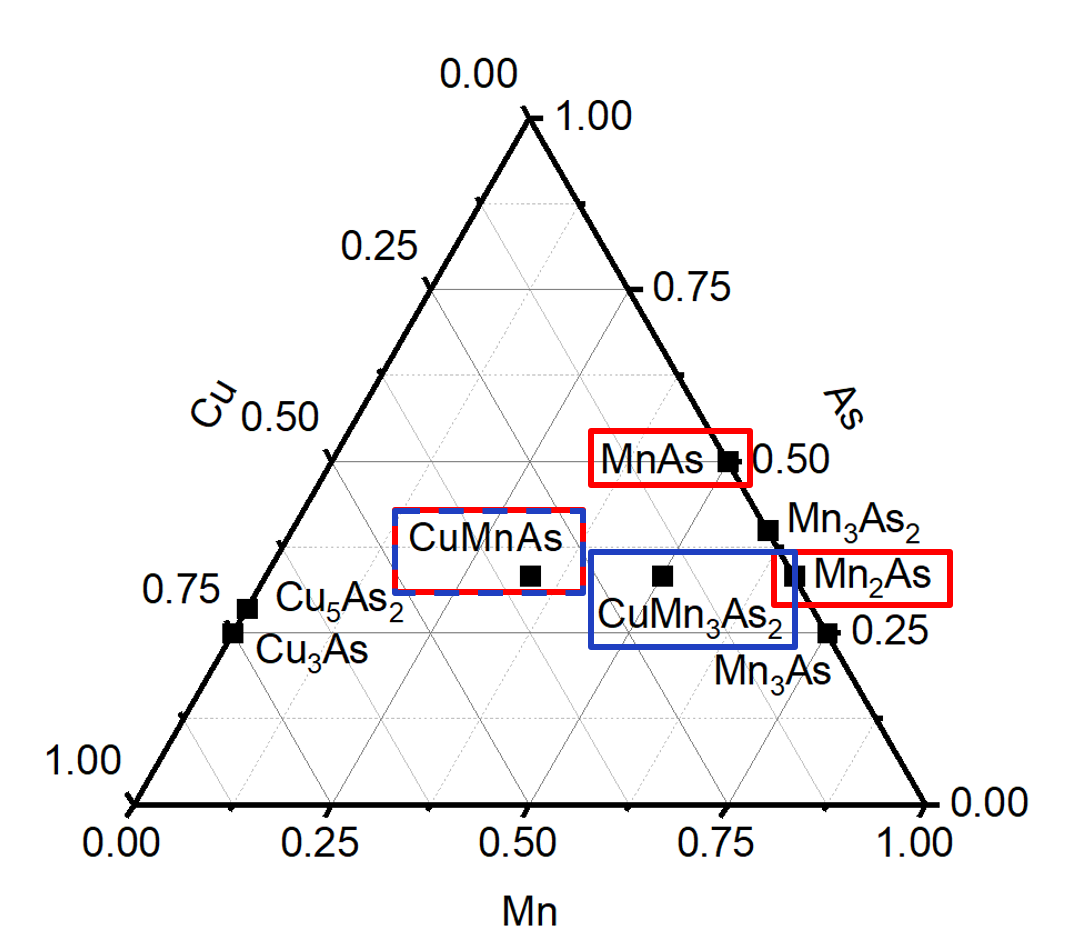
\includegraphics[width=0.8\columnwidth]{figures/ch1/Cu-Mn-As phase diagram.png} \\
\caption{\label{fig:Cu-Mn-As}
Cu-Mn-As ternary phase diagram highlighting some of the known ternary compounds in blue and known magnetic structures in red. Not all compounds in this system are shown here.
}
\end{figure}


% The dual problem
Despite the growing importance of the compounds in Cu-Mn-As system, the Cu-Mn-As ternary phase space has not been explored properly. There are four known ternary compounds including both the polymorphs of CuMnAs, orthorhombic CuMn$_3$As$_2$ and Cu$_2$Mn$_4$As$_3$ as shown in Fig. \ref{fig:Cu-Mn-As} \cite{Nateprov2011,MacA2012,Wadley2013,Uhlirova2015}. Bulk orthorhombic CuMnAs can be grown using traditional solid state synthesis routes by Cu, Mn and As powders in stoichiometric ratio and heating the powders to 1000$^\circ$C. In order to synthesize pure bulk tetragonal CuMnAs, we have to go off-stoichiometry and either substitute Mn with Cu or As \cite{Uhlirova2015}. Hence, it is important to explore different regions in the Cu-Mn-As system and verify the stability of different ternary compounds. The magnetic structures in the Cu-Mn-As system have also not been identified for most of the compounds. Apart from the four Cu-Mn-As ternary compounds, there are more than ten Mn-As binary compounds present in this system. The magnetic structures are known only for the two previously mentioned CuMnAs compounds, Mn$_2$As and MnAs as shown in Fig. \ref{fig:Cu-Mn-As} \cite{MacA2012,Wadley2013,Hills2015,Wadley2015,Austin1962,Bacon1955}. Since most, if not all, the binary Mn-As compounds are metallic, there is a need to magnetically characterize the compounds and identify their magnetic structures.

\section{Exchange interactions in Cu$_2$Sb type structures}

% Exchange interactions in Cu$_2$Sb materials.
If we want to understand the electrical switching behavior in metallic antiferromagnets, we should be able to quantify the fundamental energies such as magnetocrystalline anisotropy and exchange interactions in materials like CuMnAs. CuMnAs has a Cu$_2$Sb structure type. Other materials with this structure includes Mn$_2$As, Cr$_2$As, Fe$_2$As, CrMnAs, MnFeAs etc. \cite{Lutz-Kappelman2018,Zhang2013,Zhang2015}. Although Mn$_2$As, Cr$_2$As and Fe$_2$As have the same structure, the magnetic ground state is different in all three compounds. The strength and sign of direct exchange interactions between two magnetic atoms is a result of the nature of orbital overlap between the two magnetic atoms \cite{Zhang2013}. Since these materials are metallic, there are two contributions to indirect exchange interactions. One contribution arises from superexchange interactions mediated by As atoms and the other contribution comes from RKKY (Ruderman–Kittel–Kasuya–Yosida) interactions \cite{Zhang2015}. It is important that we are able to determine what spin interactions are relevant and how does it affect the magnetic ordering in these materials. It is also crucial that we are able to verify the computational methods and the exchange coupling values obtained from these methods so that we can use these methods for other systems as well.

%chapter 2
\chapter{Theory of electrical switching in metallic antiferromagnets}

%Introduction
Electrical switching in any magnetic compound is a series of events involving current induced spin polarization (CISP) of charge carriers and different components of CISP exerting different torque on the magnetic moments of the atoms. The nature of CISP is set by the crystal symmetry. In previous studies of CuMnAs and Mn$_2$Au, it was stated that the compound should globally centrosymmetric but locally non-centrosymmetric and the two sublattices should be related to each other by a center of inversion \cite{Zelezny2014,Zelezny2017,Wadley2016}. Is this a necessary condition for observing a staggered spin polarization configuration and can it be applied to general cases? These are some of the questions we will answer in this chapter. Once we have determined the required symmetry criteria, we will filter out metallic antiferromagnetic candidates from large databases of materials such as MPDS (Materials Platform for Data Science) and ASM (ASM International), and analyze the effect of torque on the order parameter.

\section{Hidden spin polarization in centrosymmetric crystals}

% Explanation of R2-D2 effect
It has been known for quite some time that in materials (even non-magnetic) having large spin orbit coupling (SOC) and lacking a center of inversion, magnetic fields are induced. When materials possess structural inversion asymmetry such as in quantum wells and other heterostructures, this effect is called the Rashba effect and it results in a helical type spin texture. When this occurs in materials that lack bulk inversion symmetry, the effect is called the Dresselhaus effect and it results in a unique spin texture \cite{Zhang2014}. Zhang \emph{et al.} \cite{Zhang2014} argued that since SOC is a relativistic effect, instead of considering the symmetry of the entire unit cell, one should check for atomic site symmetry to understand SOC induced spin polarization. Based on this argument, there are four cases possible as shown in Table \ref{tab:RD_effect}.

R1 and D1 effects refer to conventional Rashba and Dresselhaus spin polarization respectively. In materials that are globally centrosymmetric, hidden spin polarization is possible. There is local spin polarization near non-centrosymmetric sites but when summed over the entire unit cell, the net spin polarization is zero. This effect is called the R2 or D2 effect corresponding to Rashba or Dresselhaus effect, respectively in centrosymmetric crystals. The total spin polarization of the unit cell is the vector sum of all the local spin polarizations in the unit cell. Non-centrosymmetric point groups can be further divided into polar and non-polar groups. Local Rashba effect requires the presence of polar point groups on atomic sites and the local Dresselhaus effect requires the presence of non-polar point groups at the atom site. The presence of local spin polarization in centrosymmetric crystals opens the avenue to studying spin polarization in a larger group of compounds including metallic antiferromagnets.

\renewcommand{\arraystretch}{1.2}
\begin{table}
\caption{\label{tab:RD_effect} 
Different cases of spin polarization depending on the symmetry of atomic sites and the unit cell \cite{Zhang2014}.}
\centering
\begin{tabular}{>{\raggedright\arraybackslash}p{5cm}>{\raggedright\arraybackslash}p{3cm}>{\raggedright\arraybackslash}p{3cm}>{\raggedright\arraybackslash}p{3cm}}
\hline\hline
\textbf{} & \textbf{All non-polar point groups} & \textbf{At least one polar point groups} & \textbf{All centrosymmetric point groups}\\
\hline
\textbf{Non-Centrosymmetric space group} & D1 effect & R1/D1 effect & Not possible\\
\hline
\textbf{Centrosymmetric space group} & D2 effect & R2/D2 effect & No spin polarization\\
\hline\hline
\end{tabular}
~\\
\end{table}

\section{Finding metallic antiferromagnetic candidates with R2-D2 effect}

% Replace this figure maybe
\begin{figure}
\centering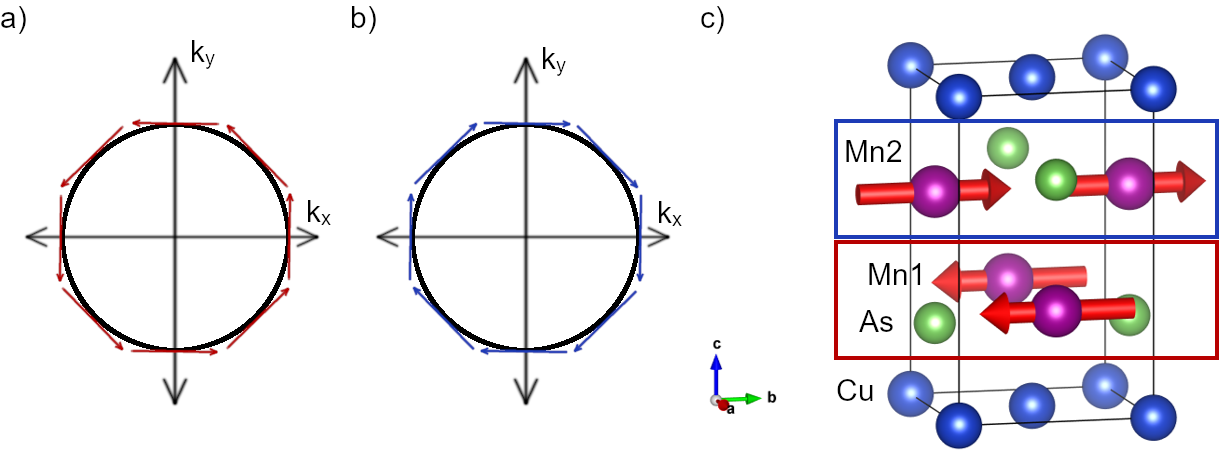
\includegraphics[width=\columnwidth]{figures/ch2/wadley_1.png} \\
\caption{\label{fig:wadley_1}
The Fermi surface of the local sectors near Mn1 and Mn2 atoms are shown in (a) and (b), respectively. The magnetic structure of tetragonal CuMnAs is shown in (c).
}
\end{figure}

% Explain use of Zunger paper in CuMnAs

In spin orbit torque based switching of metallic antiferromagnets, the same arguments apply as before except that we only care about the point group symmetry at the magnetic atom sites. For example, the magnetic structure of CuMnAs is shown in Fig. \ref{fig:wadley_1}(c). Cu and As atoms have no moments and sit on D$_{2d}$ and C$_{4v}$ sites respectively. Since only the Mn atoms have moments, we must take the site symmetry of Mn atoms into consideration. Mn atom sites have C$_{4v}$ point group symmetry which is polar. As seen in Fig. \ref{fig:wadley_1}(a,b), the Fermi surface corresponding to the Mn layer would have a Rashba-like spin texture. When current is applied, there is a spin polarization of the conduction electrons near Mn sites  which, through exchange coupling with Mn atoms, torques the order parameter. From the example of CuMnAs above, we can search for compounds from databases that are antiferromagnets or are likely to be antiferromagnets where the magnetic atoms sit on a polar point group. Such a search can be made for compounds which are not complicated by the presence of many magnetic sites with different point groups. The general case applicable for all magnetic compounds will be considered in the following sections. Following is the general procedure for extracting potential metallic antiferromagnet candidates from databases -

% Procedure list
\begin{enumerate}
\item Search for known metallic antiferromagnets from database having tetragonal, trigonal or hexagonal crystal system.
\item Remove duplicate and non-centrosymmetric compounds.
\item Identify the Néel temperature and magnetic ordering.
\item Filter out compounds having Néel temperature $>$ 300 K.
\item Identify the nature of atomic site symmetry and select compounds.
\item Study available literature to see if any compounds can be synthesized as single crystals.
\end{enumerate}

This procedure assumes that we are starting with a collection of known or possible metallic antiferromagnets. This is true in case of compounds downloaded from MPDS. In case of ASM database, the compounds are metallic but their magnetism is not known beforehand. We will have to make some assumptions based on the chemical nature and stoichiometry of the ions present in the compound in order to select antiferromagnets. Tetragonal, trigonal or hexagonal crystal systems are preferred since they allow for the presence of multiple degenerate axes for N\'eel vector orientation. It is still important to check if the magnetic structure for the compound is known or not and if the N\'eel vector points along the degerate axis. Carrying out the above mentioned steps for compounds in MPDS and ASM database gives us a list of compounds that have been grouped together based on their structure types in Table \ref{tab:metallic_afm_candidates}.

\renewcommand{\arraystretch}{1.2}
\begin{table}
\caption{\label{tab:metallic_afm_candidates} 
List of metallic antiferromagnetic candidates filtered out from MPDS and ASM database and their metal atom site symmetries}
\centering
\begin{tabular}{>{\raggedright\arraybackslash}p{3cm}>{\raggedright\arraybackslash}p{4cm}>{\centering}p{3cm}>{\raggedright\arraybackslash}p{4cm}}
\hline\hline
\textbf{Structure type} & \textbf{List of compounds} & \textbf{Point group} & \textbf{Magnetism}\\
\hline
MoSi$_2$ & Mn$_2$Au, Cr$_2$Al, Ni$_2$Ta & C$_{4v}$ & Mn$_2$Au is a candidate\\
\hline
HfFe$_6$Ge$_6$ & ScFe$_6$Ge$_6$ & C$_{2v}$ & AFM with N\'eel vector along $c$\\
\hline
Mg$_3$Cd & Mn$_3$Ga, Mn$_3$Ge, Mn$_3$Sn, Fe$_3$Ga, Co$_3$Mo, Co$_3$W, Ni$_3$In, Ni$_3$Sn, Ni$_3$Zr & C$_{2v}$ & Non-collinear AFM\\
\hline
IrIn$_3$ & CoGa$_3$, CoIn$_3$, FeGa$_3$ & C$_{2v}$ & FeGa$_3$ and CoGa$_3$ are diamagnets\\
\hline
MoNi$_4$ & MoNi$_4$, WNi$_4$ & C$_{1v}$ & Unknown\\
\hline
Ni$_2$Al$_3$ & Ni$_2$Al$_3$, Ni$_2$Ga$_3$, Ni$_2$In$_3$ & C$_{3v}$ & Unknown\\
\hline\hline
\end{tabular}
~\\
\end{table}

%Discuss the list of compounds obtained

The first group of compounds consist of materials in MoSi$_2$ structure type. Mn$_2$Au is a well-known compound that has been extensively studied for electrical switching applications \cite{Meinert2018,Bodnar2019}. Cr$_2$Al powders can be prepared using traditional solid state synthesis routes by heating to above 850$^\circ$C \cite{Susner2015}. Early neutron diffraction experiments suggest Cr moments align at 65$^\circ$ to the $ab$ plane \cite{Atoji1965}. However, a later article \cite{Kallel1967} by another group of researchers indicate that the determined magnetic structure may not be correct. Regardless of whether the moments align in the $ab$ plane or not, Cr$_2$Al is an interesting candidate to study. ScFe$_6$Ge$_6$ is AFM at room temperature \cite{Venturini1992}. However, the Fe moments align along $c$ and does not satify our criteria \cite{Mazet2000}. Compounds in the Mg$_3$Cd structure type contain Kagome lattice of magnetic atoms. Mn$_3$Sn and Mn$_3$Ge are known to have a non-collinear spin arrangement. They have become popular for showing anomalous hall and spin hall effect \cite{Nakatsuji2015,Kubler2014,Kimata2019}. Electrical switching was demonstrated in Mn$_3$Sn recently. In the fourth group of compounds, both FeGa$_3$ and CoGa$_3$ are known to show diamagnetic properties and hence they can be discarded \cite{Haussermann2002,Viklund2002,Zhang2017}. The magnetism is unknown in the final two groups of compounds in MoNi$_4$ and Ni$_2$Al$_3$ structure types and most of these compounds can be synthesized by the arc melting process \cite{Harker1944,Taylor1972}.

\section{Components of torque from non-equilibrium CISP}



\section{Torque from CISP in Fe$_2$As}

\begin{figure}
\centering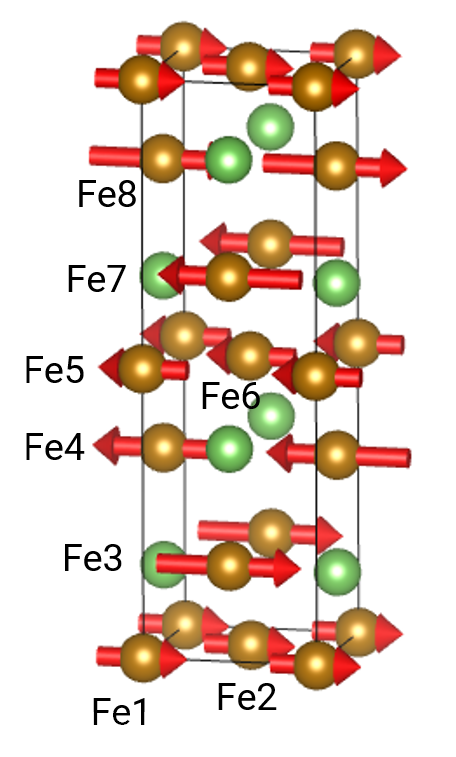
\includegraphics[width=0.3\columnwidth]{figures/ch2/Fe2As.png} \\
\caption{\label{fig:Fe2As}
Electronic band structure
}
\end{figure}

\begin{figure}
\centering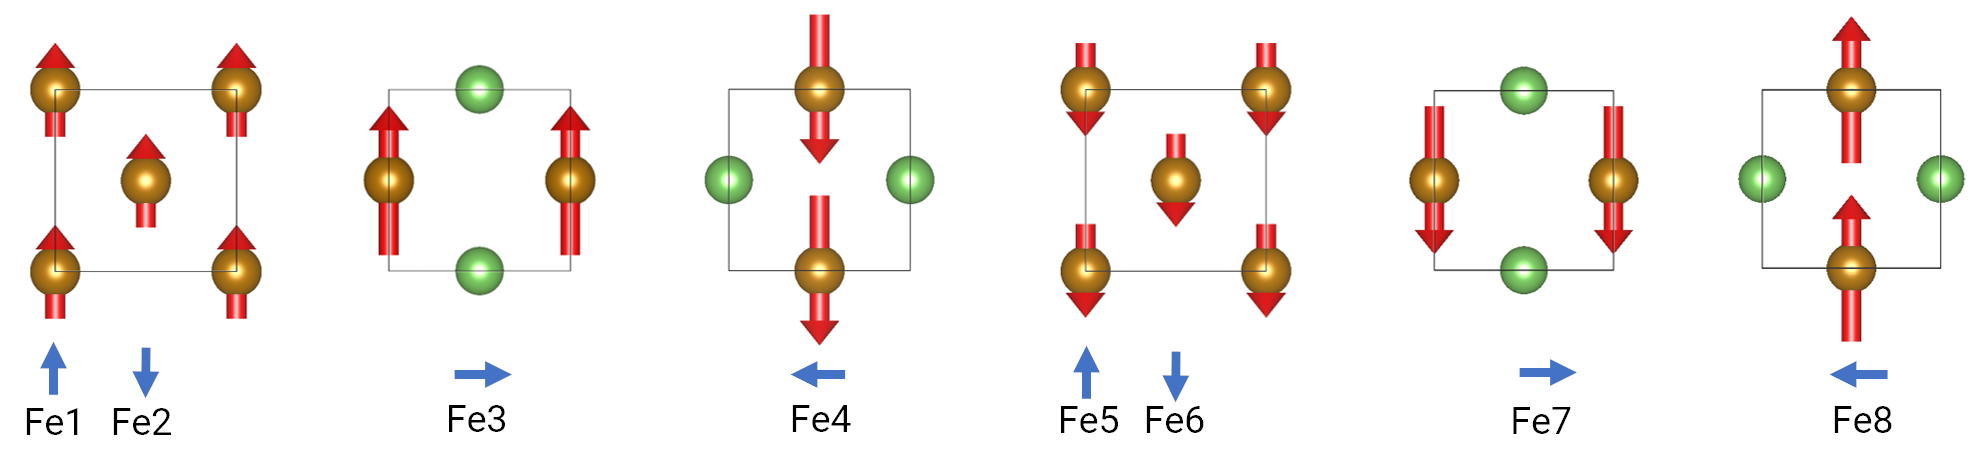
\includegraphics[width=\columnwidth]{figures/ch2/fieldlike_torque_Fe2As.png} \\
\caption{\label{fig:fieldlike_torque_Fe2As}
Electronic band structure
}
\end{figure}

\begin{figure}
\centering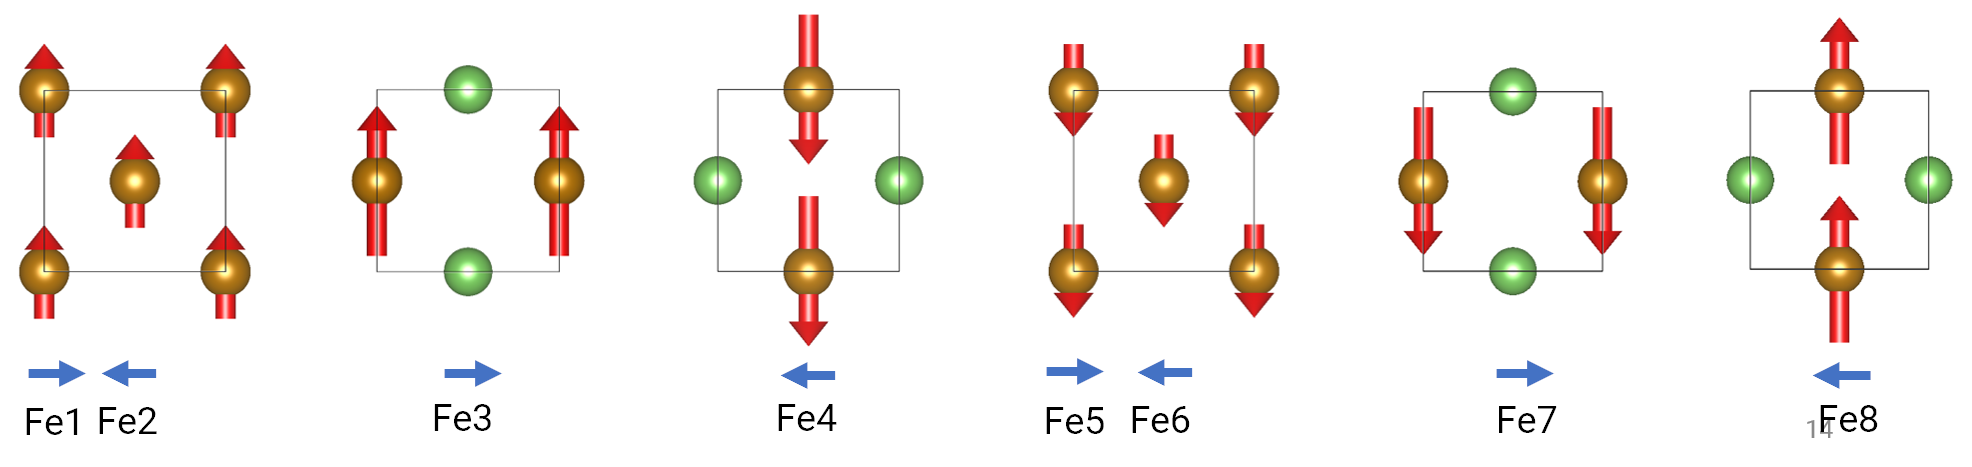
\includegraphics[width=\columnwidth]{figures/ch2/antidamping_torque_Fe2As.png} \\
\caption{\label{fig:antidamping_torque_Fe2As}
Electronic band structure
}
\end{figure}

\section{Acknowledgements}

% Acknowledge Scott and Carmen

I would like to acknowledge two REU students, Scott Berens and Carmen Paquette, for compiling the list of metallic antiferromagnets from MPDS and ASM databases respectively. It saved me a lot of time and I was able to analyze the symmetry requirements on a much smaller list of compounds.

%chapter 3
\chapter{Magnetic structure refinement from neutron diffraction measurements}

\begin{figure}
\centering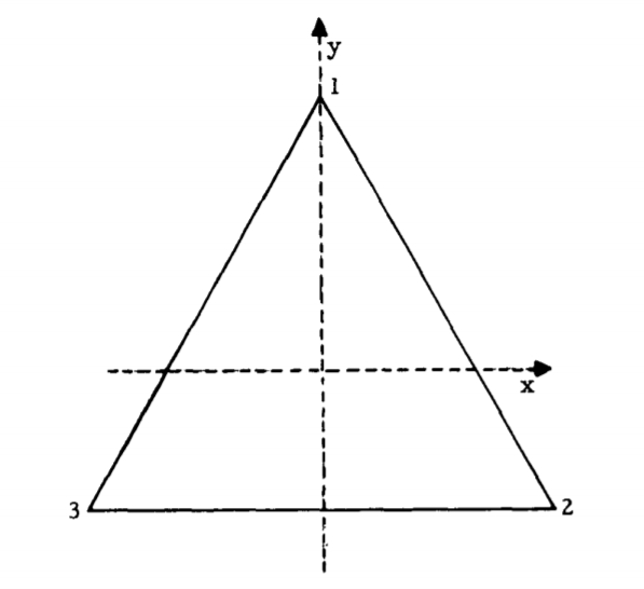
\includegraphics[width=0.5\columnwidth]{figures/ch3/C3v.png} \\
\caption{\label{fig:C3v}
Electronic band structure
}
\end{figure}

\begin{figure}
\centering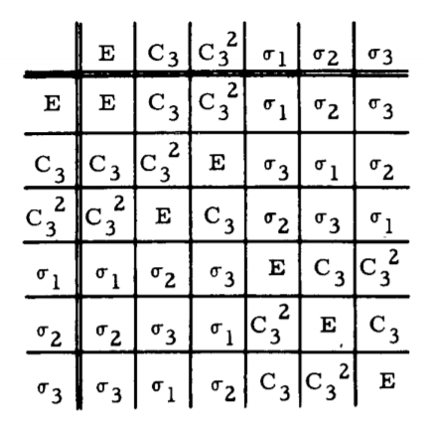
\includegraphics[width=0.5\columnwidth]{figures/ch3/group_multiplication_table_C3v.png} \\
\caption{\label{fig:gmt_C3v}
Electronic band structure
}
\end{figure}

\begin{figure}
\centering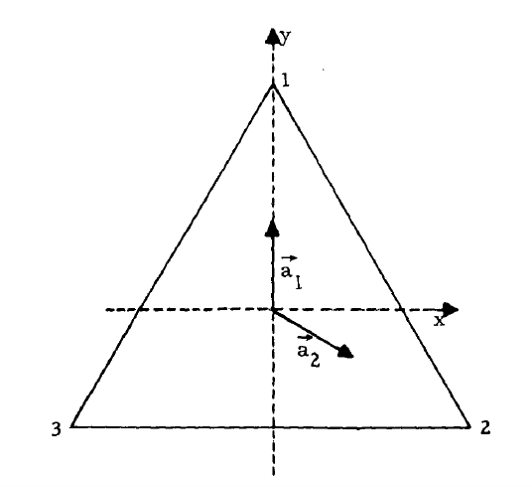
\includegraphics[width=0.5\columnwidth]{figures/ch3/C3v_a1_a2.png} \\
\caption{\label{fig:C3v_a1_a2}
Electronic band structure
}
\end{figure}

\begin{figure}
\centering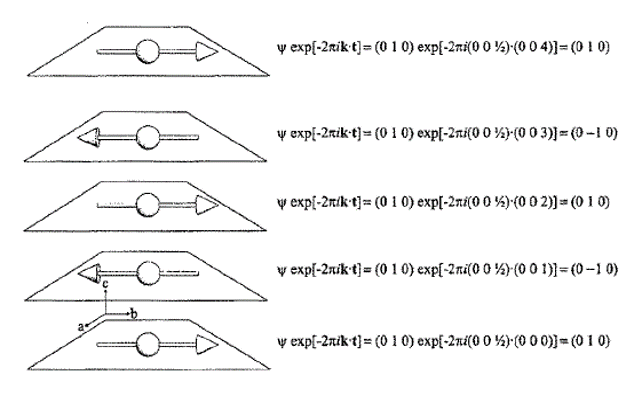
\includegraphics[width=\columnwidth]{figures/ch3/propagation_vector.png} \\
\caption{\label{fig:propagation_vector}
Electronic band structure
}
\end{figure}

\begin{figure}
\centering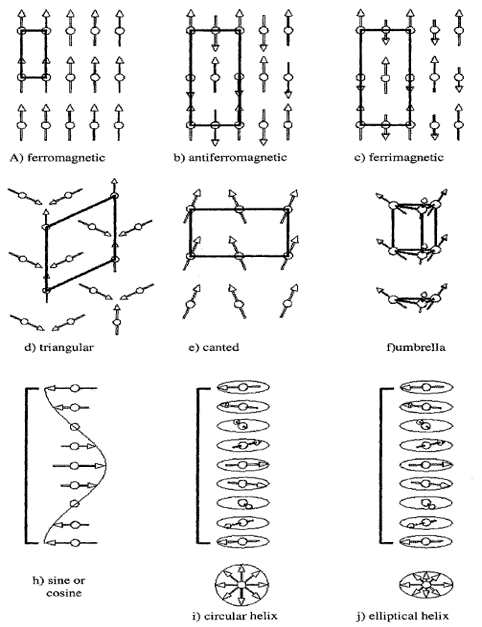
\includegraphics[width=\columnwidth]{figures/ch3/mag_structures_single_k.png} \\
\caption{\label{fig:mag_structures_single_k}
Electronic band structure
}
\end{figure}

\begin{figure}
\centering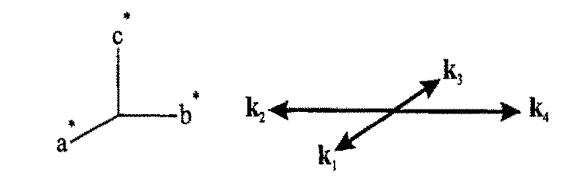
\includegraphics[width=0.7\columnwidth]{figures/ch3/star_of_propagation_vector_k.png} \\
\caption{\label{fig:star}
Electronic band structure
}
\end{figure}

\begin{figure}
\centering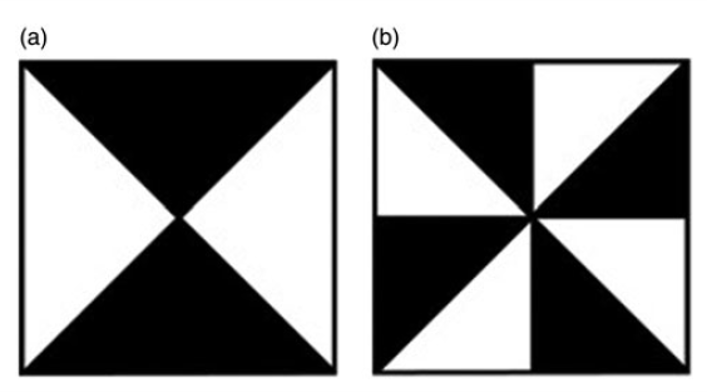
\includegraphics[width=0.5\columnwidth]{figures/ch3/symmetry_based_analysis.png} \\
\caption{\label{fig:symmetry_based_analysis}
Electronic band structure
}
\end{figure}

\Blindtext[6]

%chapter 4
\chapter{Materials synthesis and characterization}

This is a citation to~\cite{Walker2015} and~\cite{Hager2006}.

\begin{figure}
\centering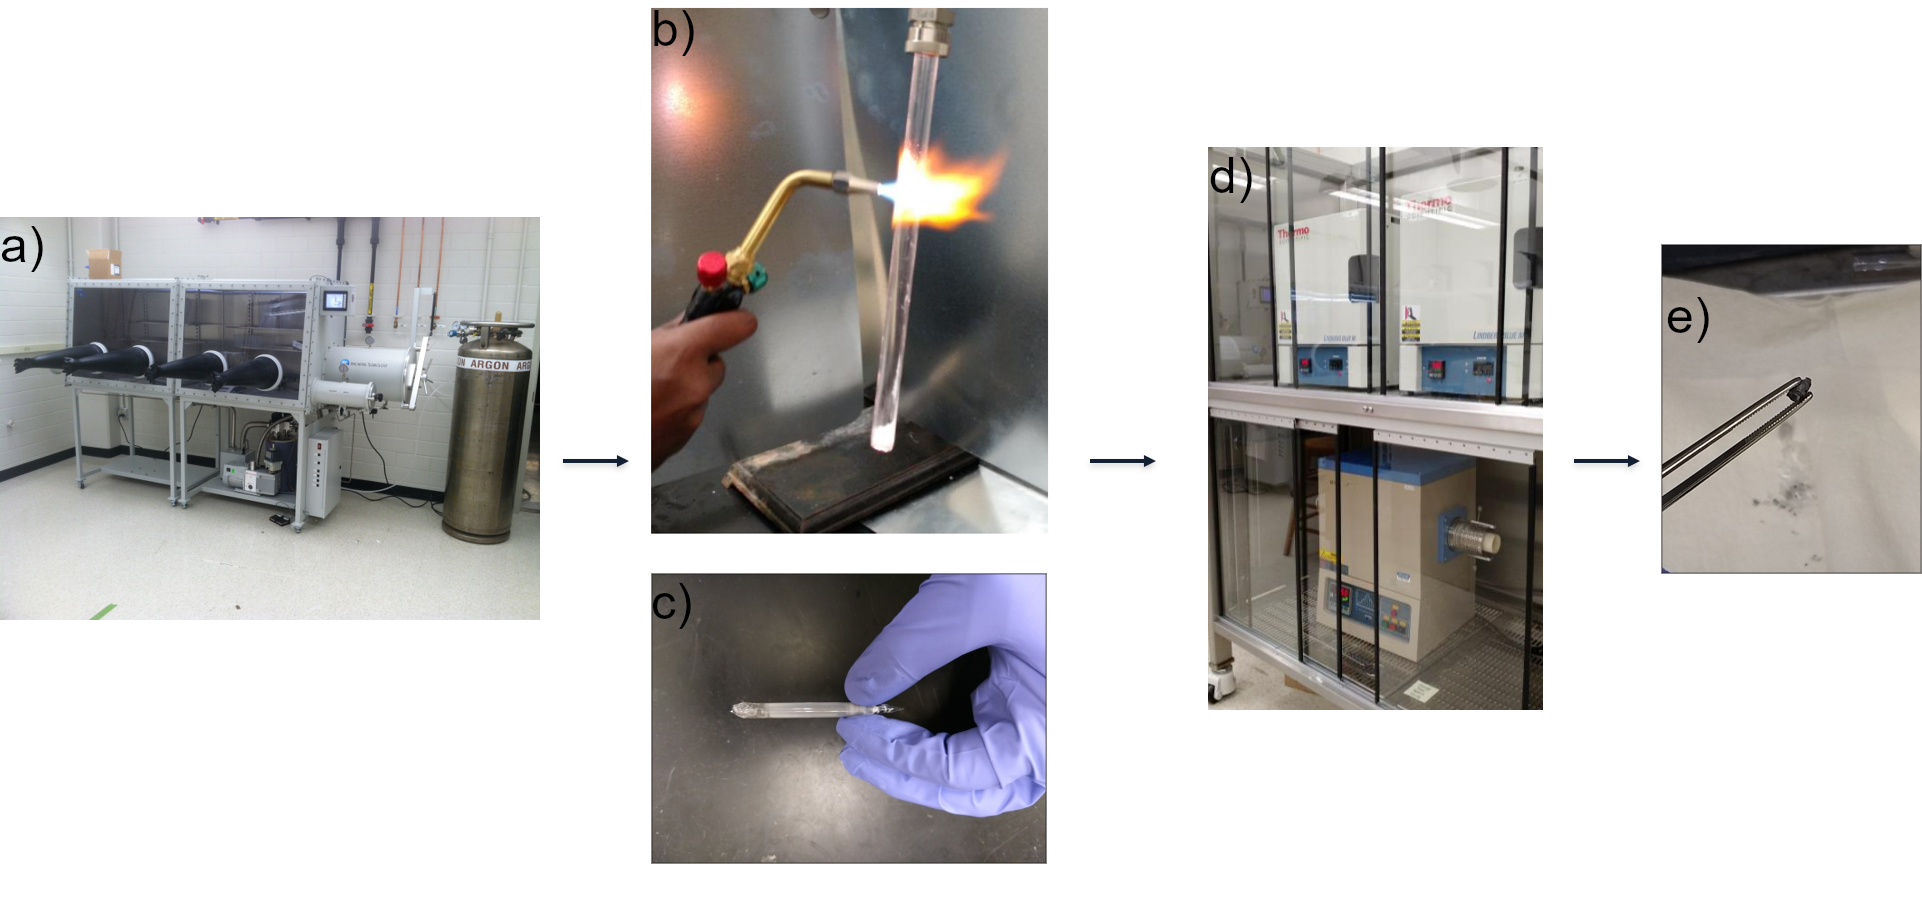
\includegraphics[width=\columnwidth]{figures/ch4/synthesis_procedure.png} \\
\caption{\label{fig:synthesis_procedure}
Electronic band structure
}
\end{figure}

%chapter 5
\chapter{Discovery and magnetic frustration of hexagonal Cu$_{0.82}$Mn$_{1.18}$As}

\begin{figure}
\centering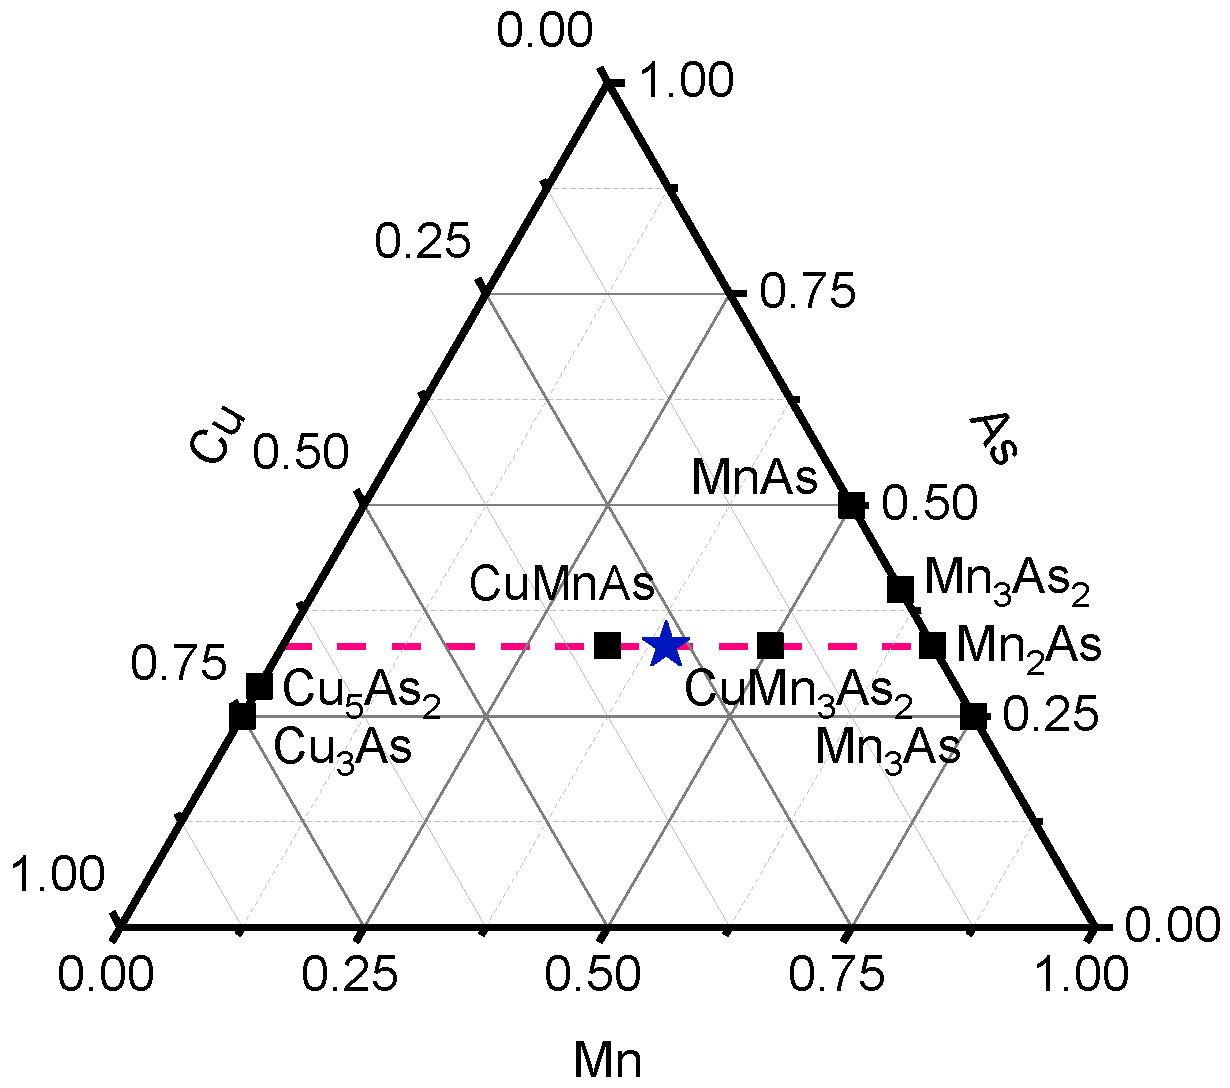
\includegraphics[width=\columnwidth]{figures/ch5/phase_diagram_cropped.pdf} \\
\caption{\label{fig:phase_diagram}
Electronic band structure
}
\end{figure}

\begin{figure}
\centering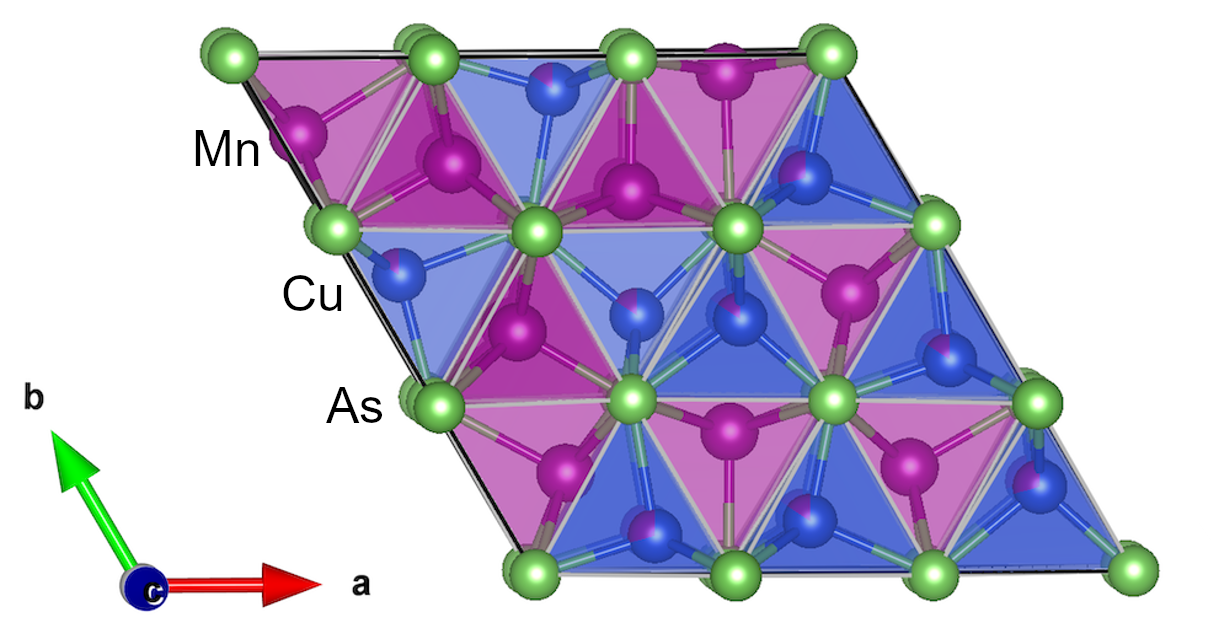
\includegraphics[width=\columnwidth]{figures/ch5/CuMnAs_chemical_structure.png} \\
\caption{\label{fig:chemical_structure}
Electronic band structure
}
\end{figure}

\begin{figure}
\centering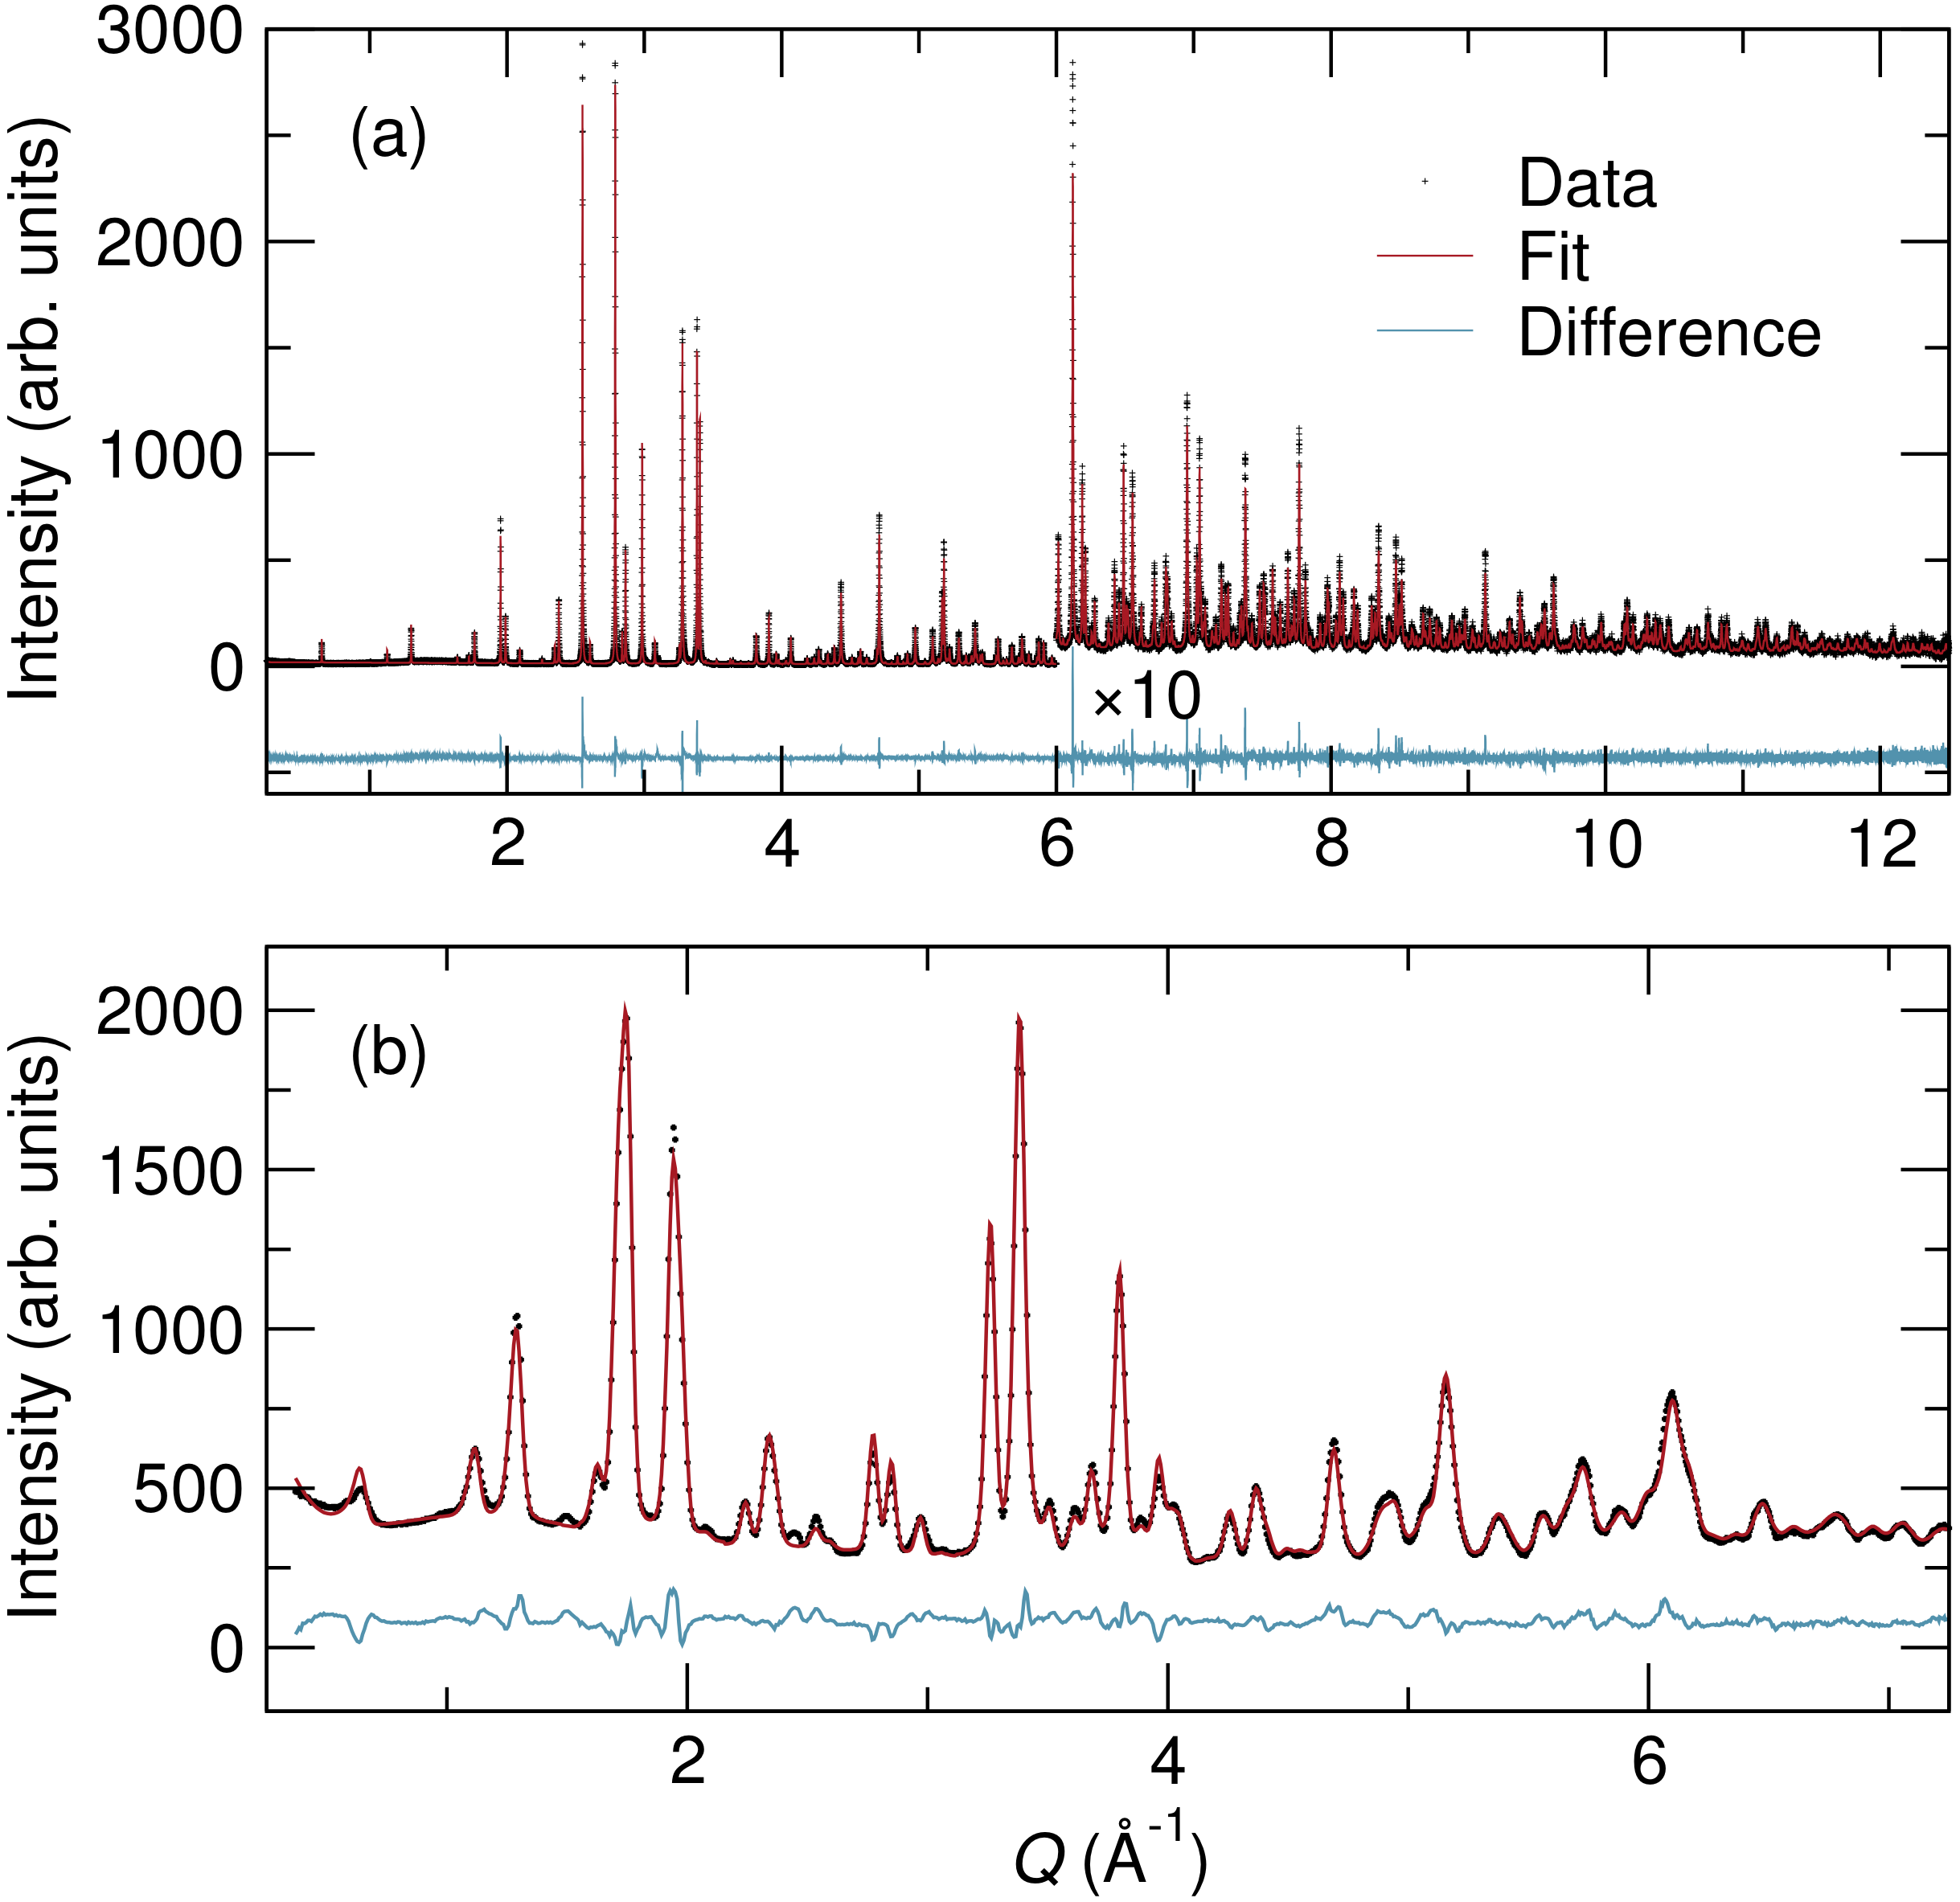
\includegraphics[width=\columnwidth]{figures/ch5/h-cumnas_11bm_100k_wand_400k_combine.png} \\
\caption{\label{fig:11BM_WAND}
Electronic band structure
}
\end{figure}

\begin{figure}
\centering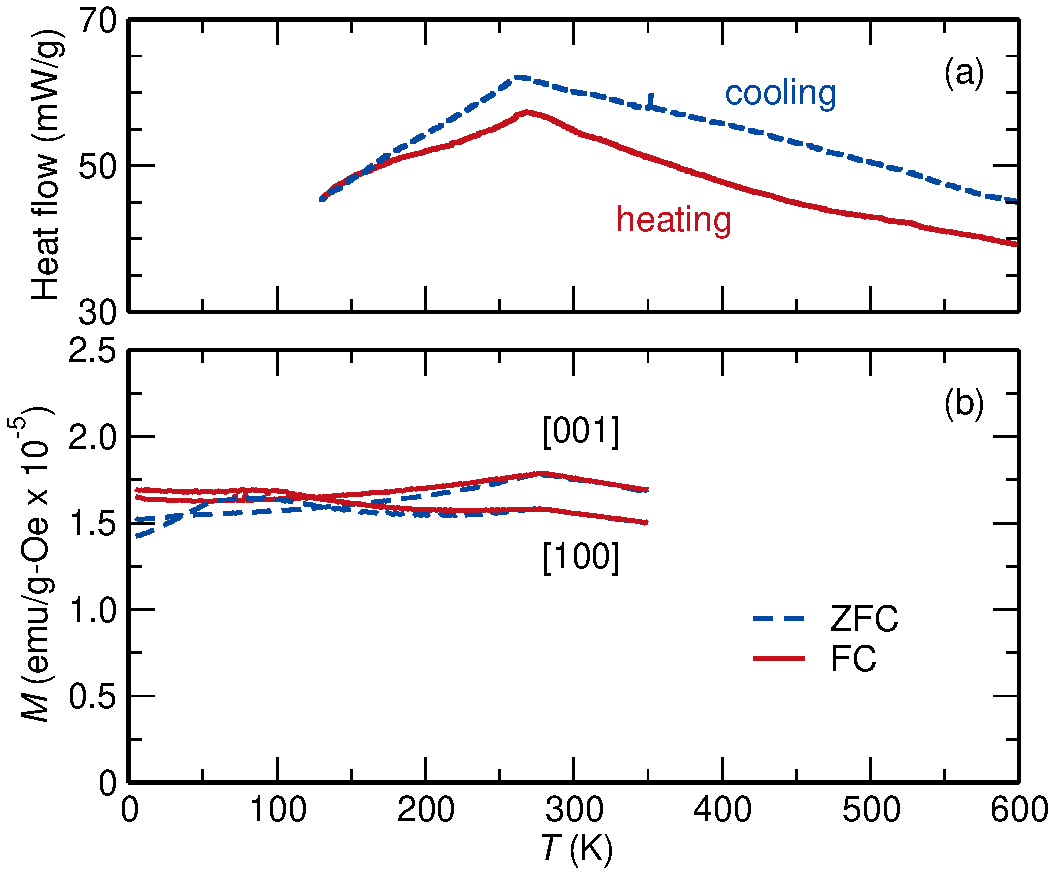
\includegraphics[width=\columnwidth]{figures/ch5/dsc-mpms_norm_cropped.pdf} \\
\caption{\label{fig:dsc_mpms}
Electronic band structure
}
\end{figure}

\begin{figure}
\centering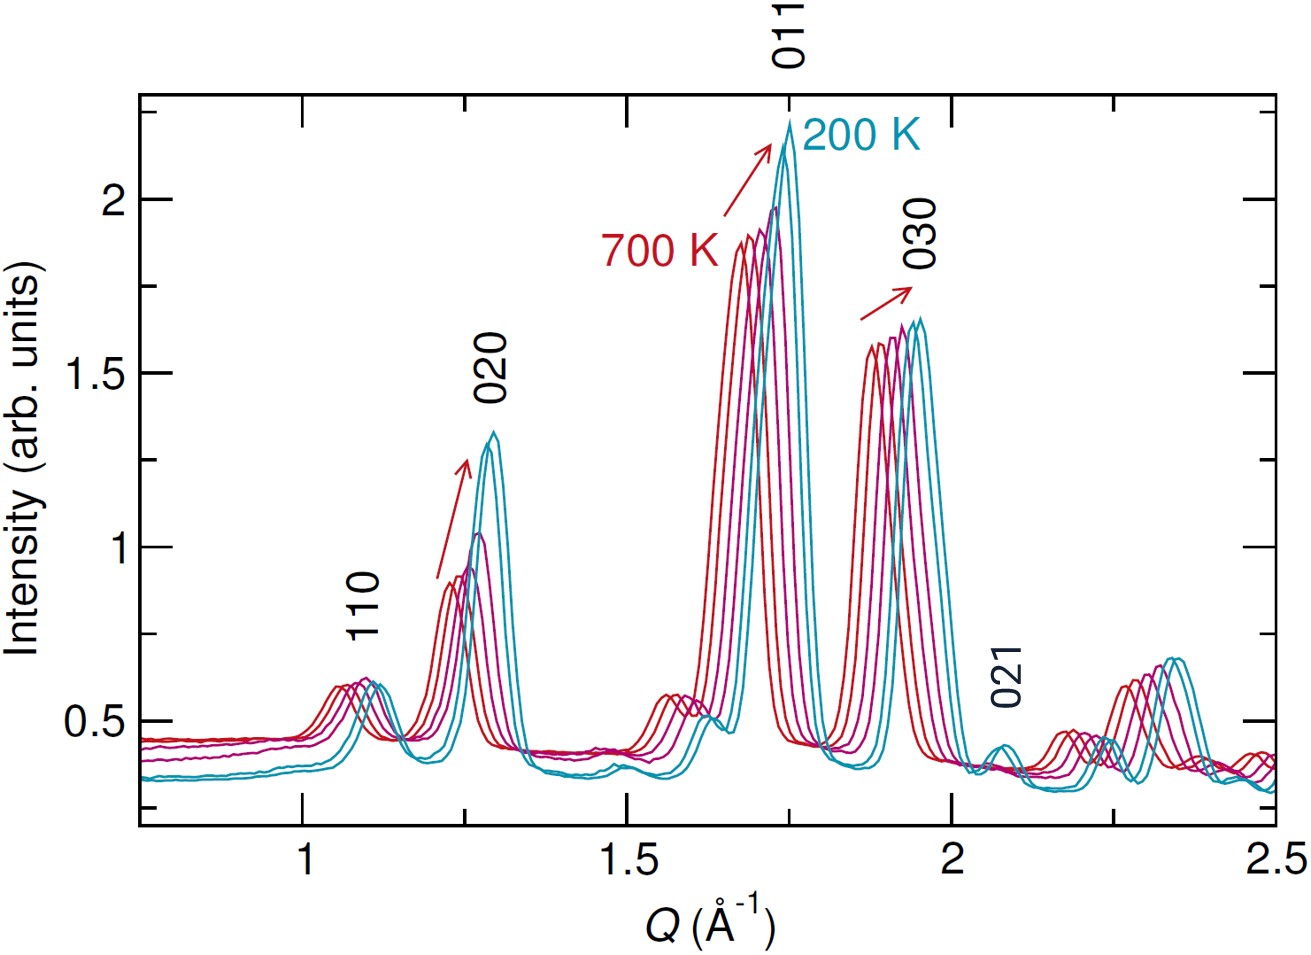
\includegraphics[width=\columnwidth]{figures/ch5/WAND_data.png} \\
\caption{\label{fig:WAND_data}
Electronic band structure
}
\end{figure}

\begin{figure}
\centering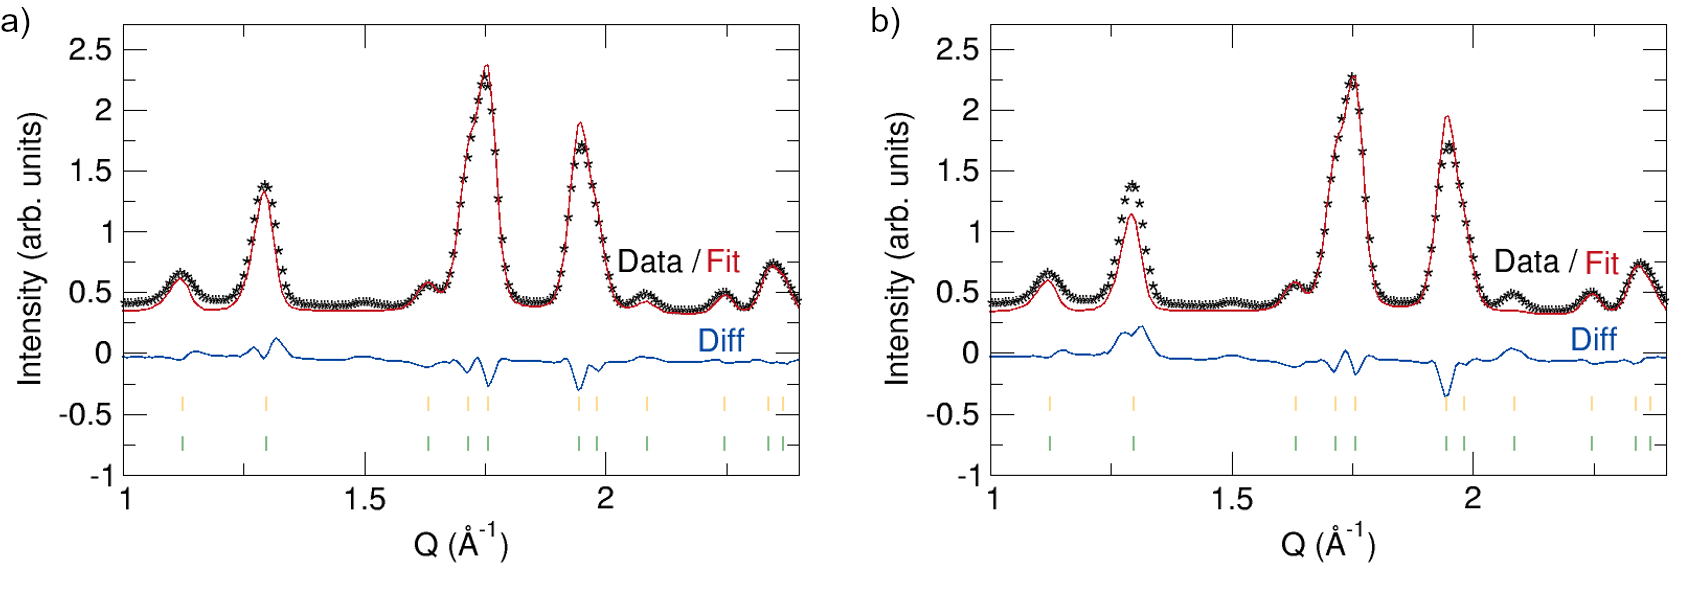
\includegraphics[width=\columnwidth]{figures/ch5/wand_refinement.png} \\
\caption{\label{fig:wand_refinement}
Electronic band structure
}
\end{figure}

\begin{figure}
\centering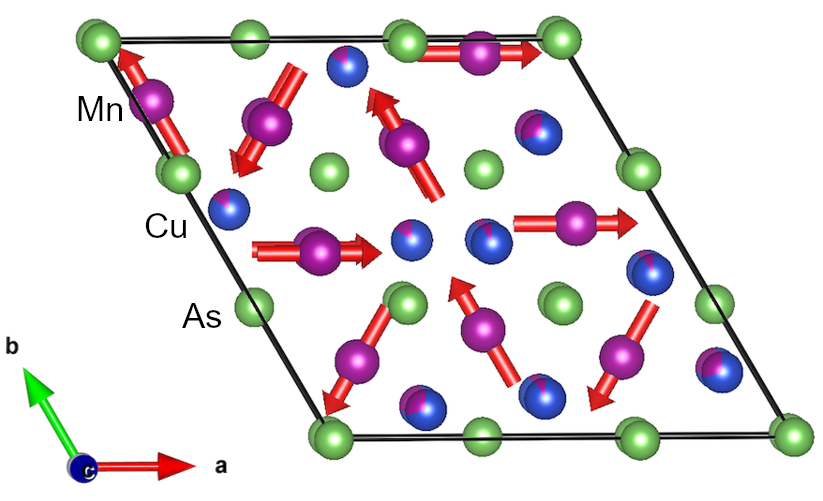
\includegraphics[width=\columnwidth]{figures/ch5/CuMnAs_magnetic_structure.png} \\
\caption{\label{fig:CuMnAs_magnetic_structure}
Electronic band structure
}
\end{figure}

\begin{figure}
\centering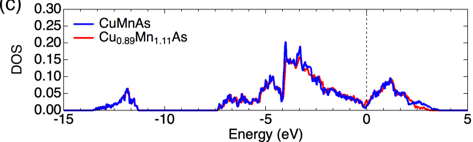
\includegraphics[width=\columnwidth]{figures/ch5/DOS_CuMnAs.png} \\
\caption{\label{fig:DOS}
Electronic band structure
}
\end{figure}

\begin{figure}
\centering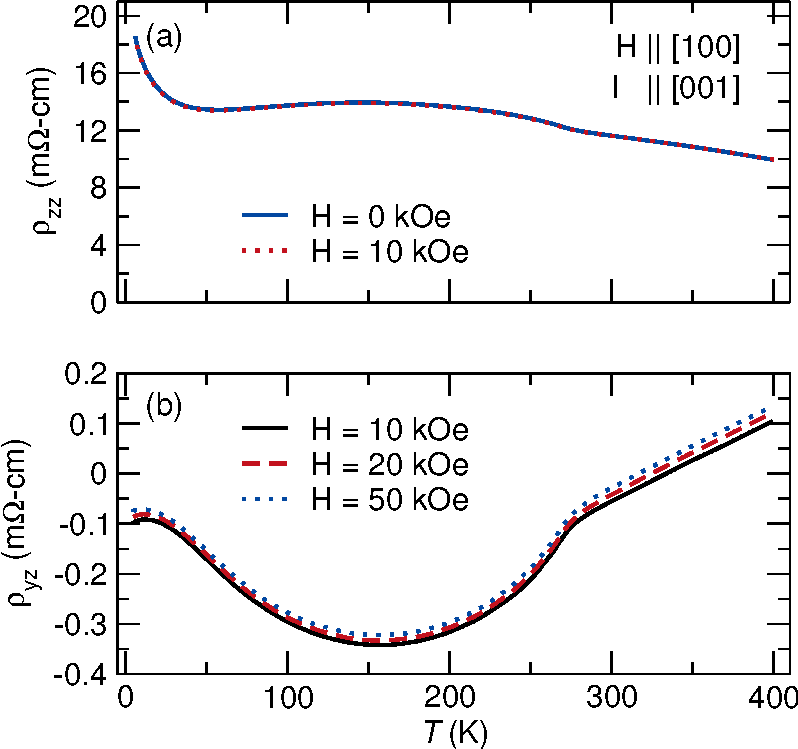
\includegraphics[width=\columnwidth]{figures/ch5/resistivity_data_hall_cropped.pdf} \\
\caption{\label{fig:resistivity}
Electronic band structure
}
\end{figure}

\Blindtext[6]

%chapter 6
\chapter{Two step magnetic ordering in monoclinic Mn$_3$As$_2$}

\begin{figure}
\centering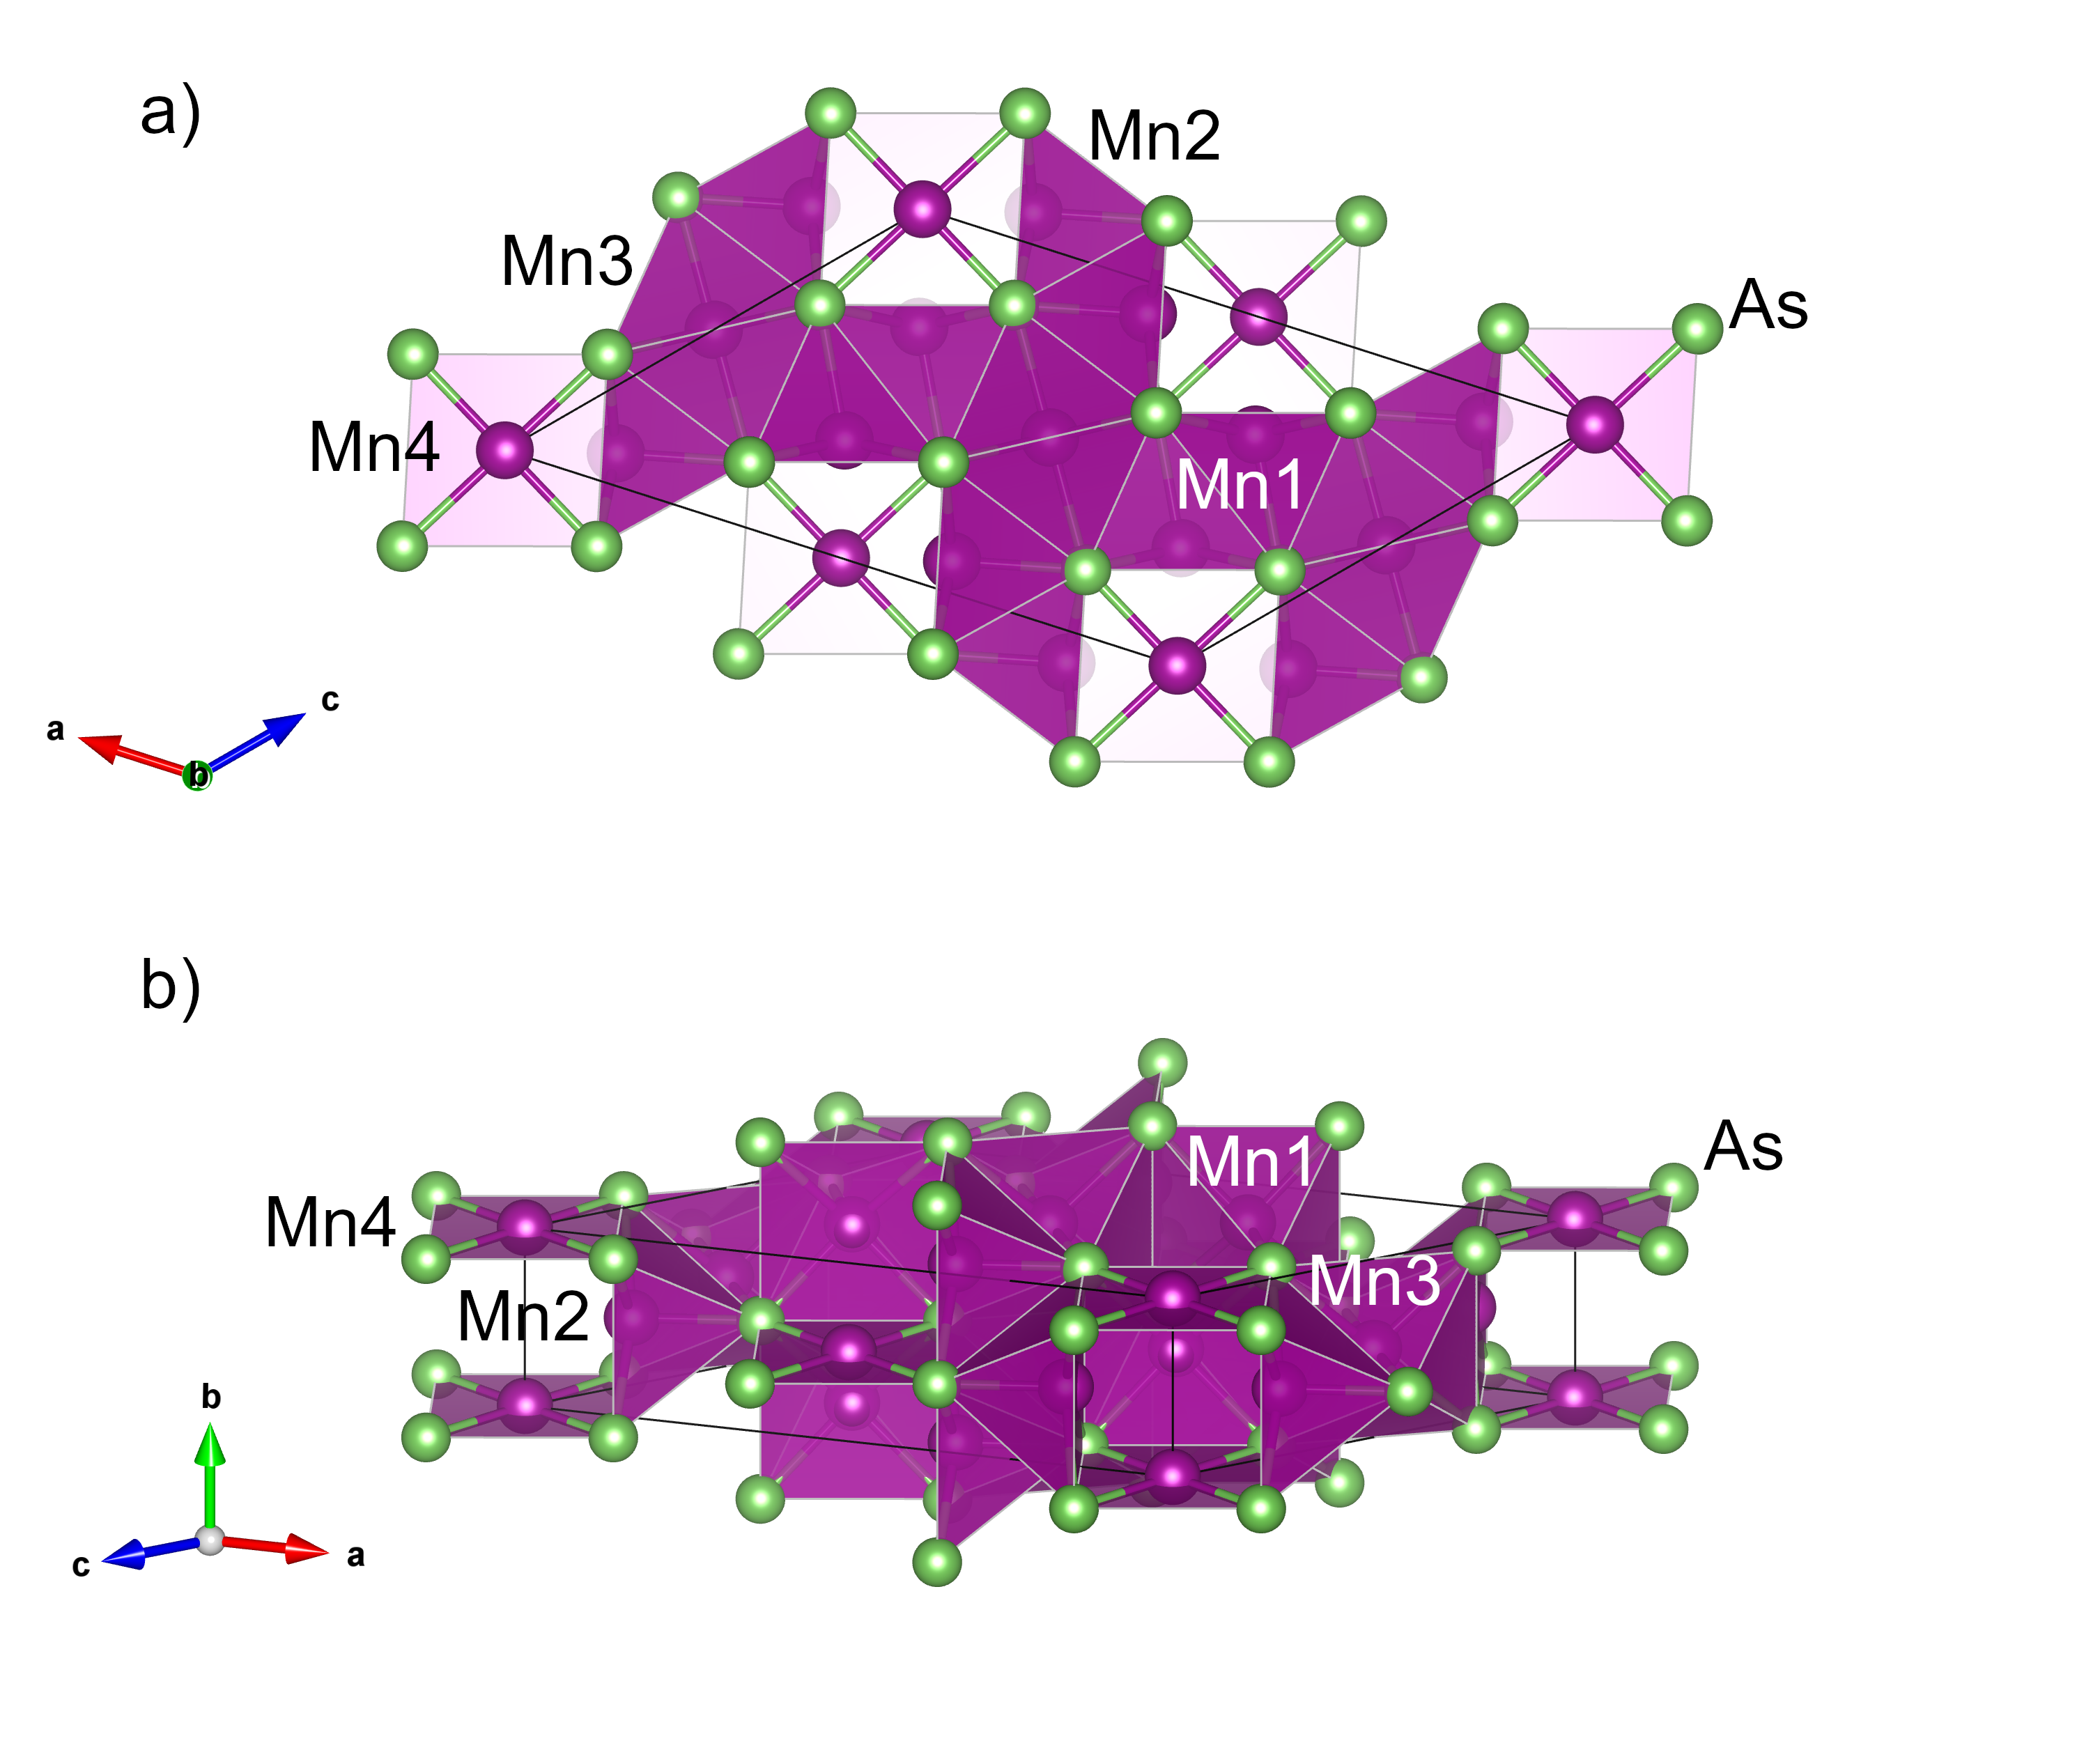
\includegraphics[width=\columnwidth]{figures/ch6/monoclinic_Mn3As2_75510.png} \\
\caption{\label{fig:Mn3As2}
Electronic band structure
}
\end{figure}

\begin{figure}
\centering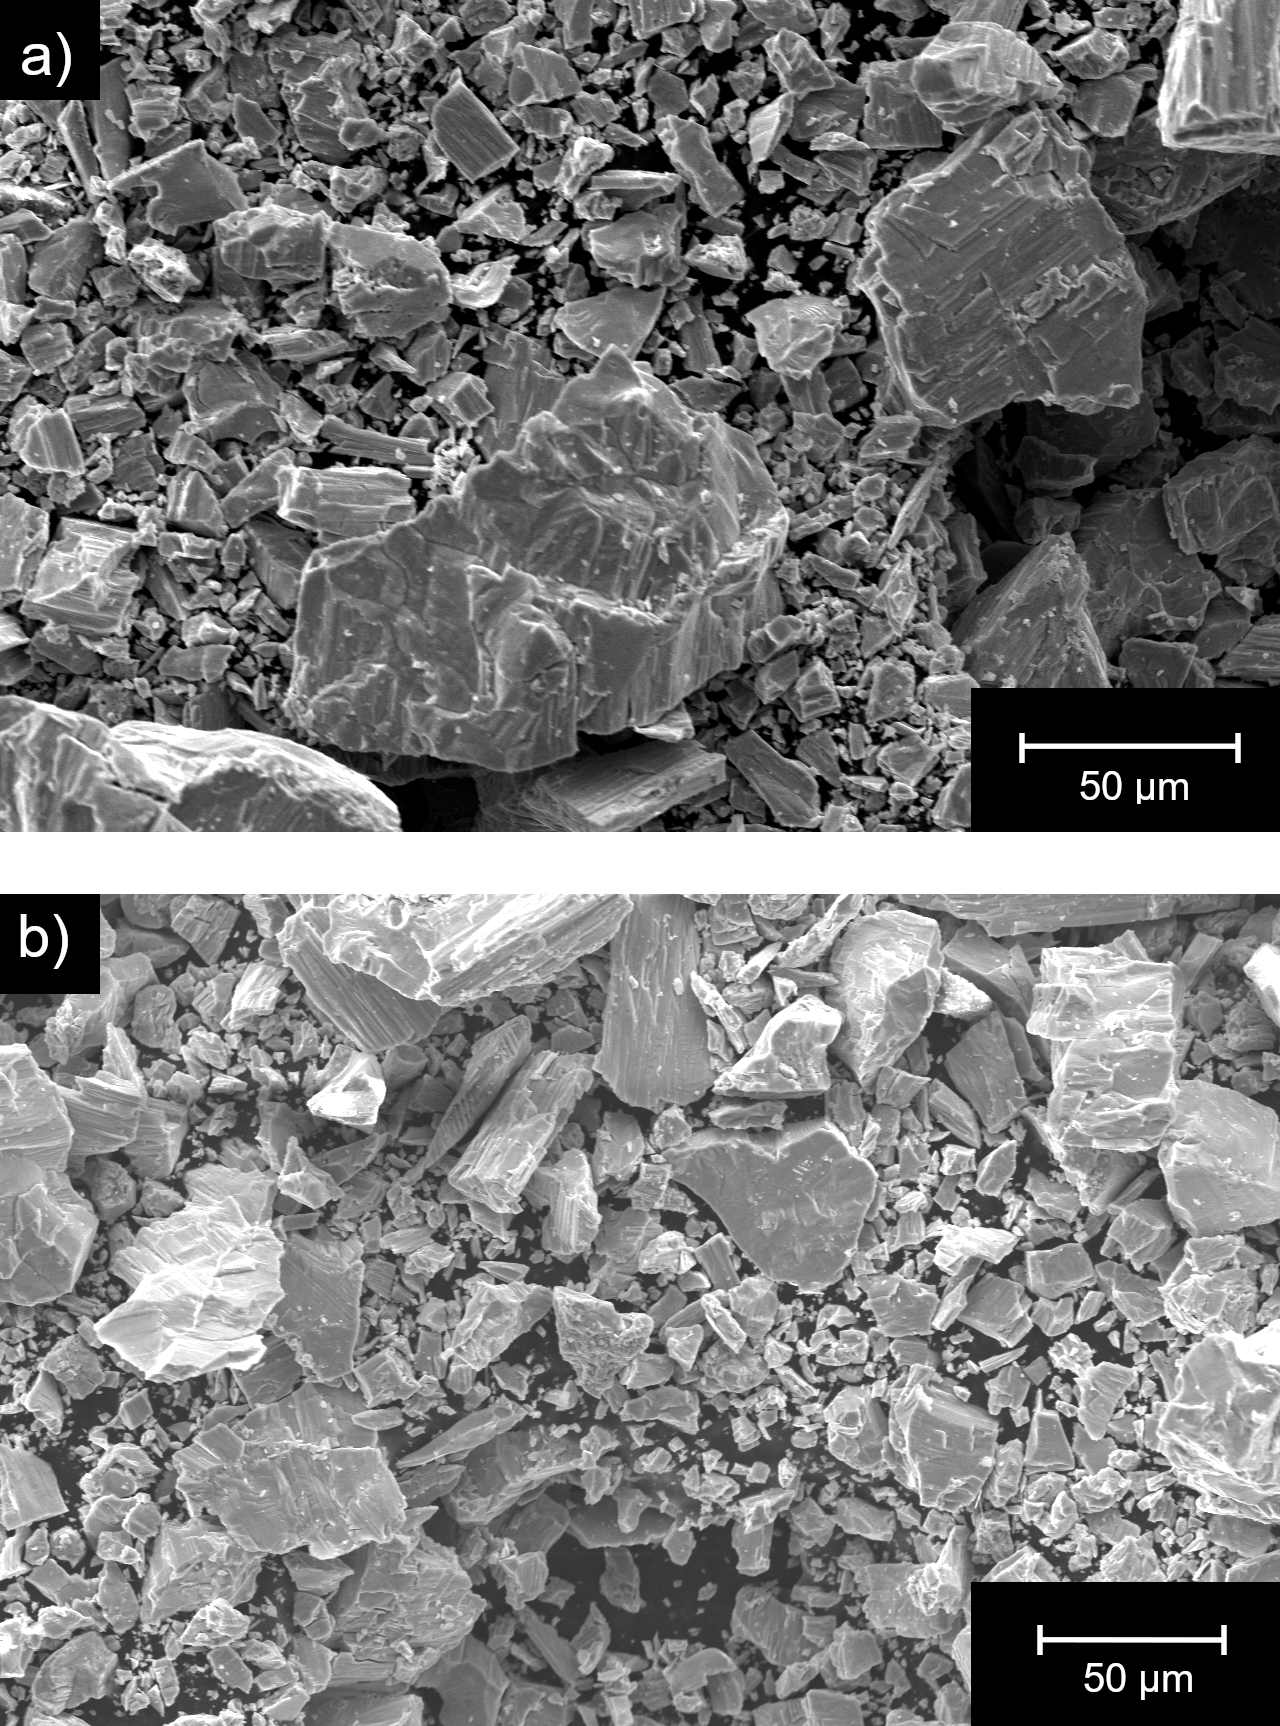
\includegraphics[width=0.5\columnwidth]{figures/ch6/Mn3As2_SEM_image.png} \\
\caption{\label{fig:Mn3As2_SEM}
Electronic band structure
}
\end{figure}

\begin{figure}
\centering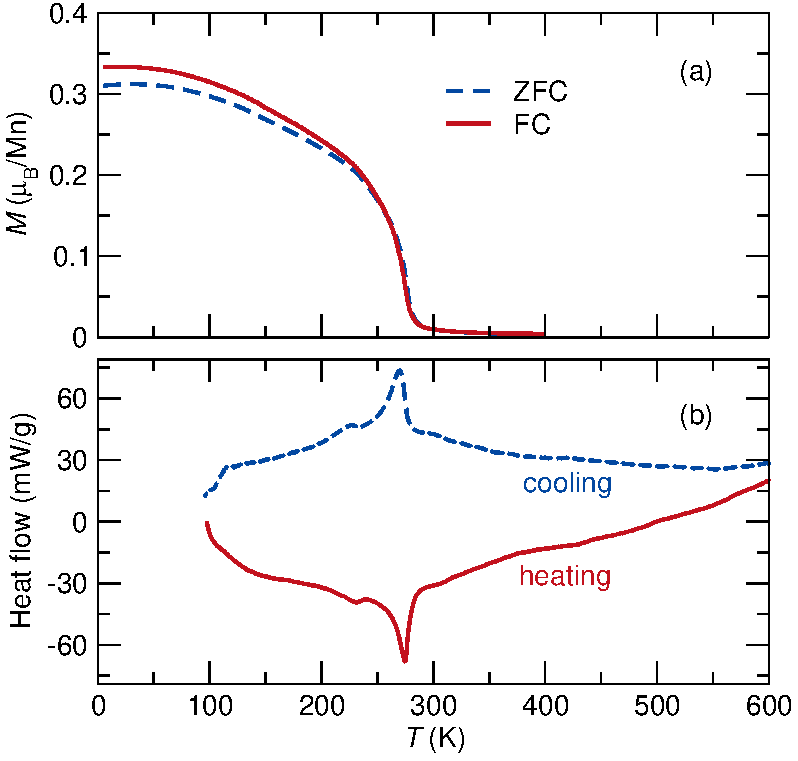
\includegraphics[width=\columnwidth]{figures/ch6/FC_ZFC_DSC_Mn3As2_cropped.pdf} \\
\caption{\label{fig:Mn3As2_FC_ZFC_DSC}
Electronic band structure
}
\end{figure}

\begin{figure}
\centering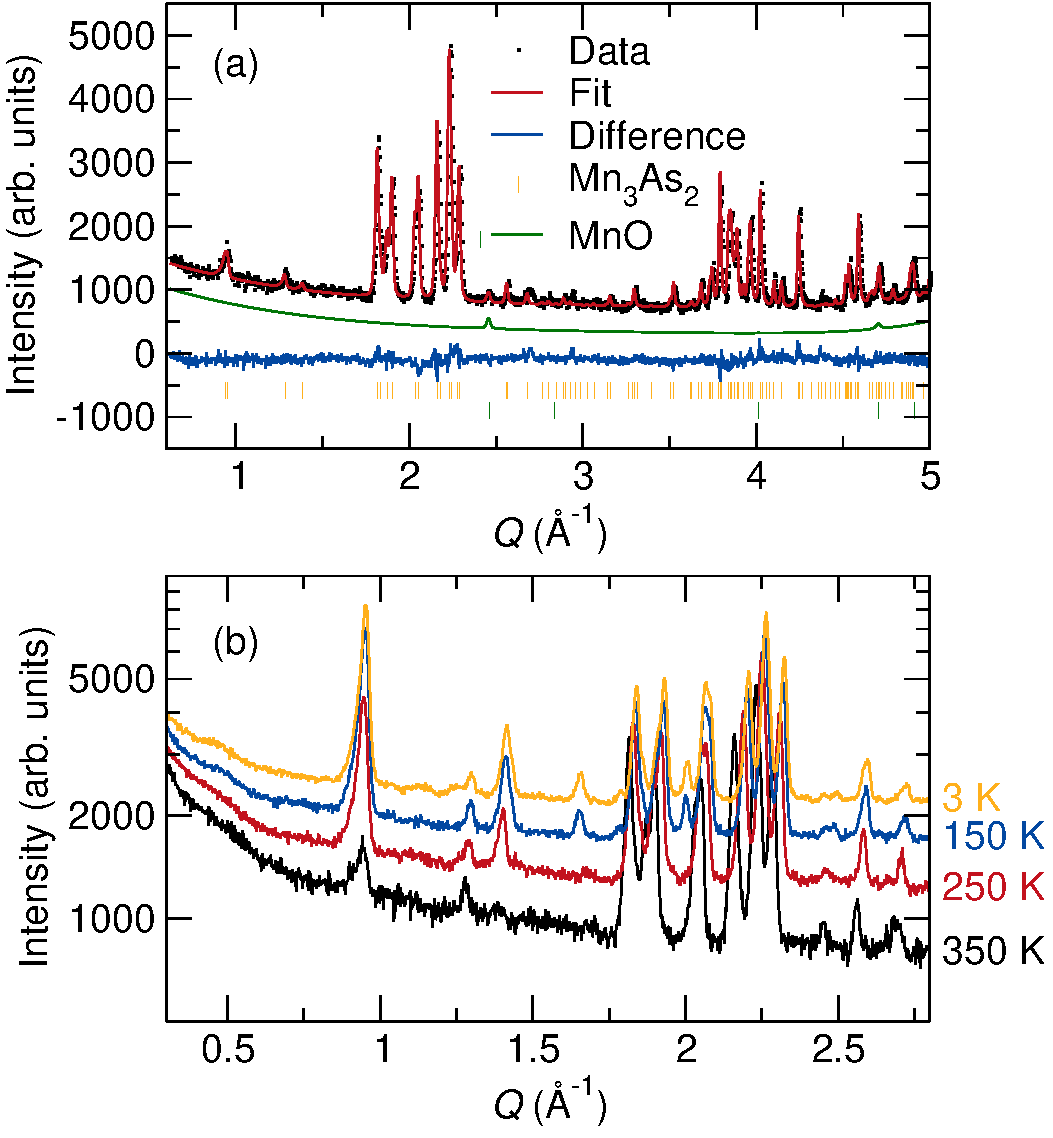
\includegraphics[width=\columnwidth]{figures/ch6/350K_rietveld_diff_temp_NPD_cropped.pdf} \\
\caption{\label{fig:350K}
Electronic band structure
}
\end{figure}

\begin{figure}
\centering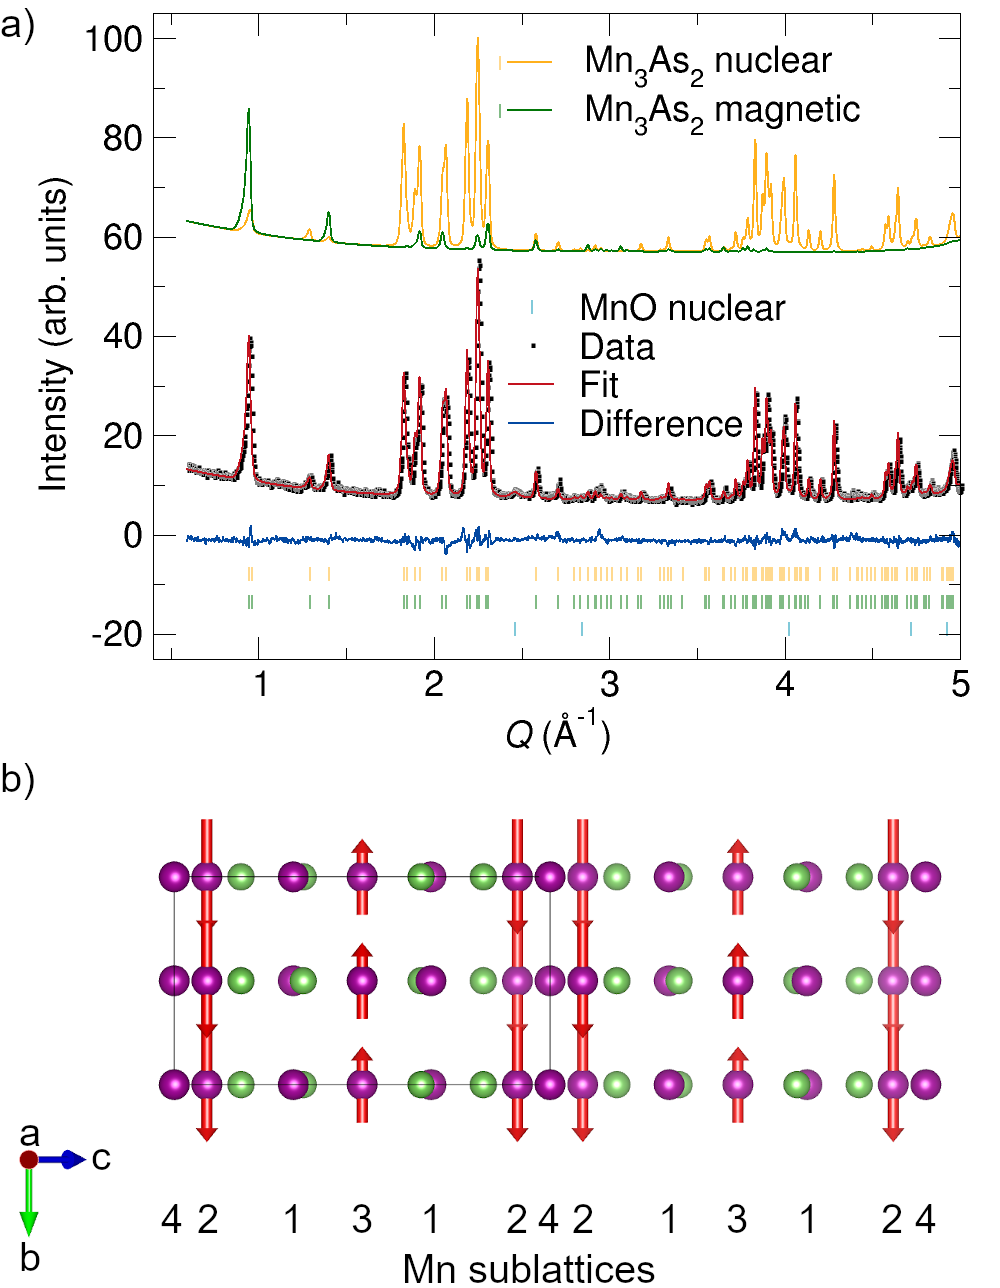
\includegraphics[width=\columnwidth]{figures/ch6/250K_mag_structure.png} \\
\caption{\label{fig:250K}
Electronic band structure
}
\end{figure}


\begin{figure}
\centering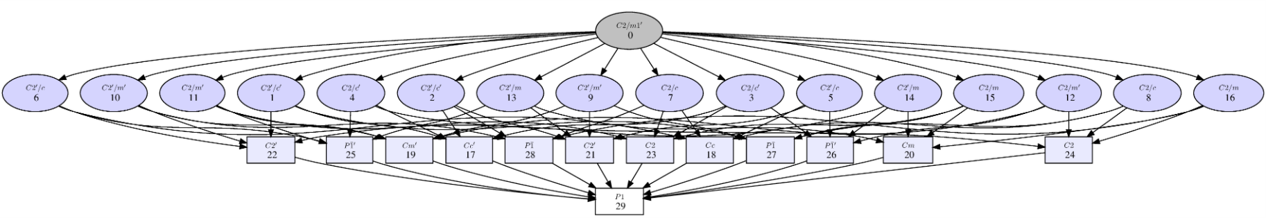
\includegraphics[width=\columnwidth]{figures/ch6/graph_of_subgraphs_3K.png} \\
\caption{\label{fig:subgraphs}
Electronic band structure
}
\end{figure}

\begin{figure}
\centering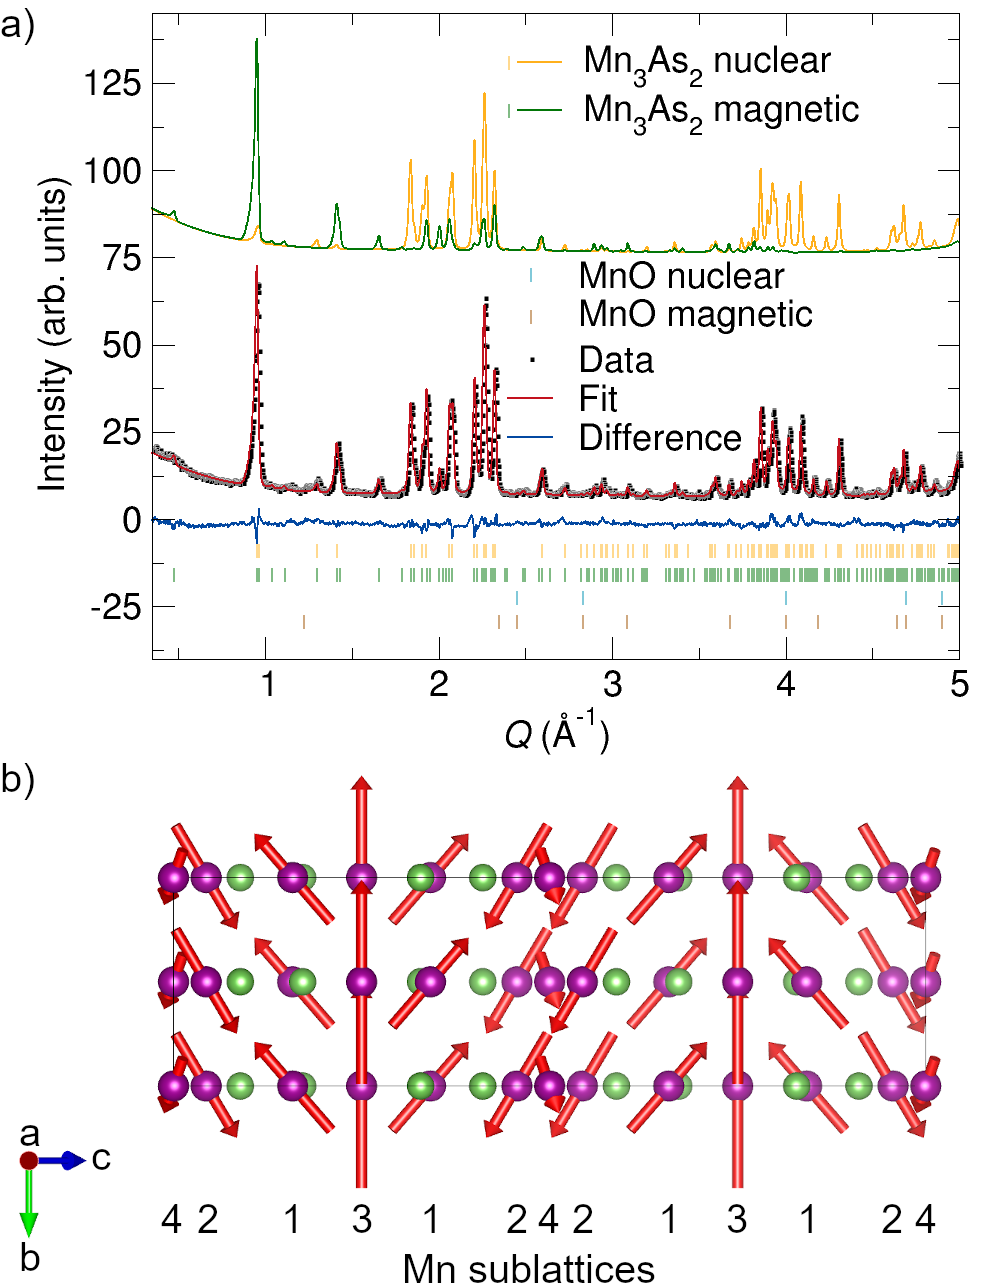
\includegraphics[width=\columnwidth]{figures/ch6/3K_mag_structure.png} \\
\caption{\label{fig:3K}
Electronic band structure
}
\end{figure}


\begin{figure}
\centering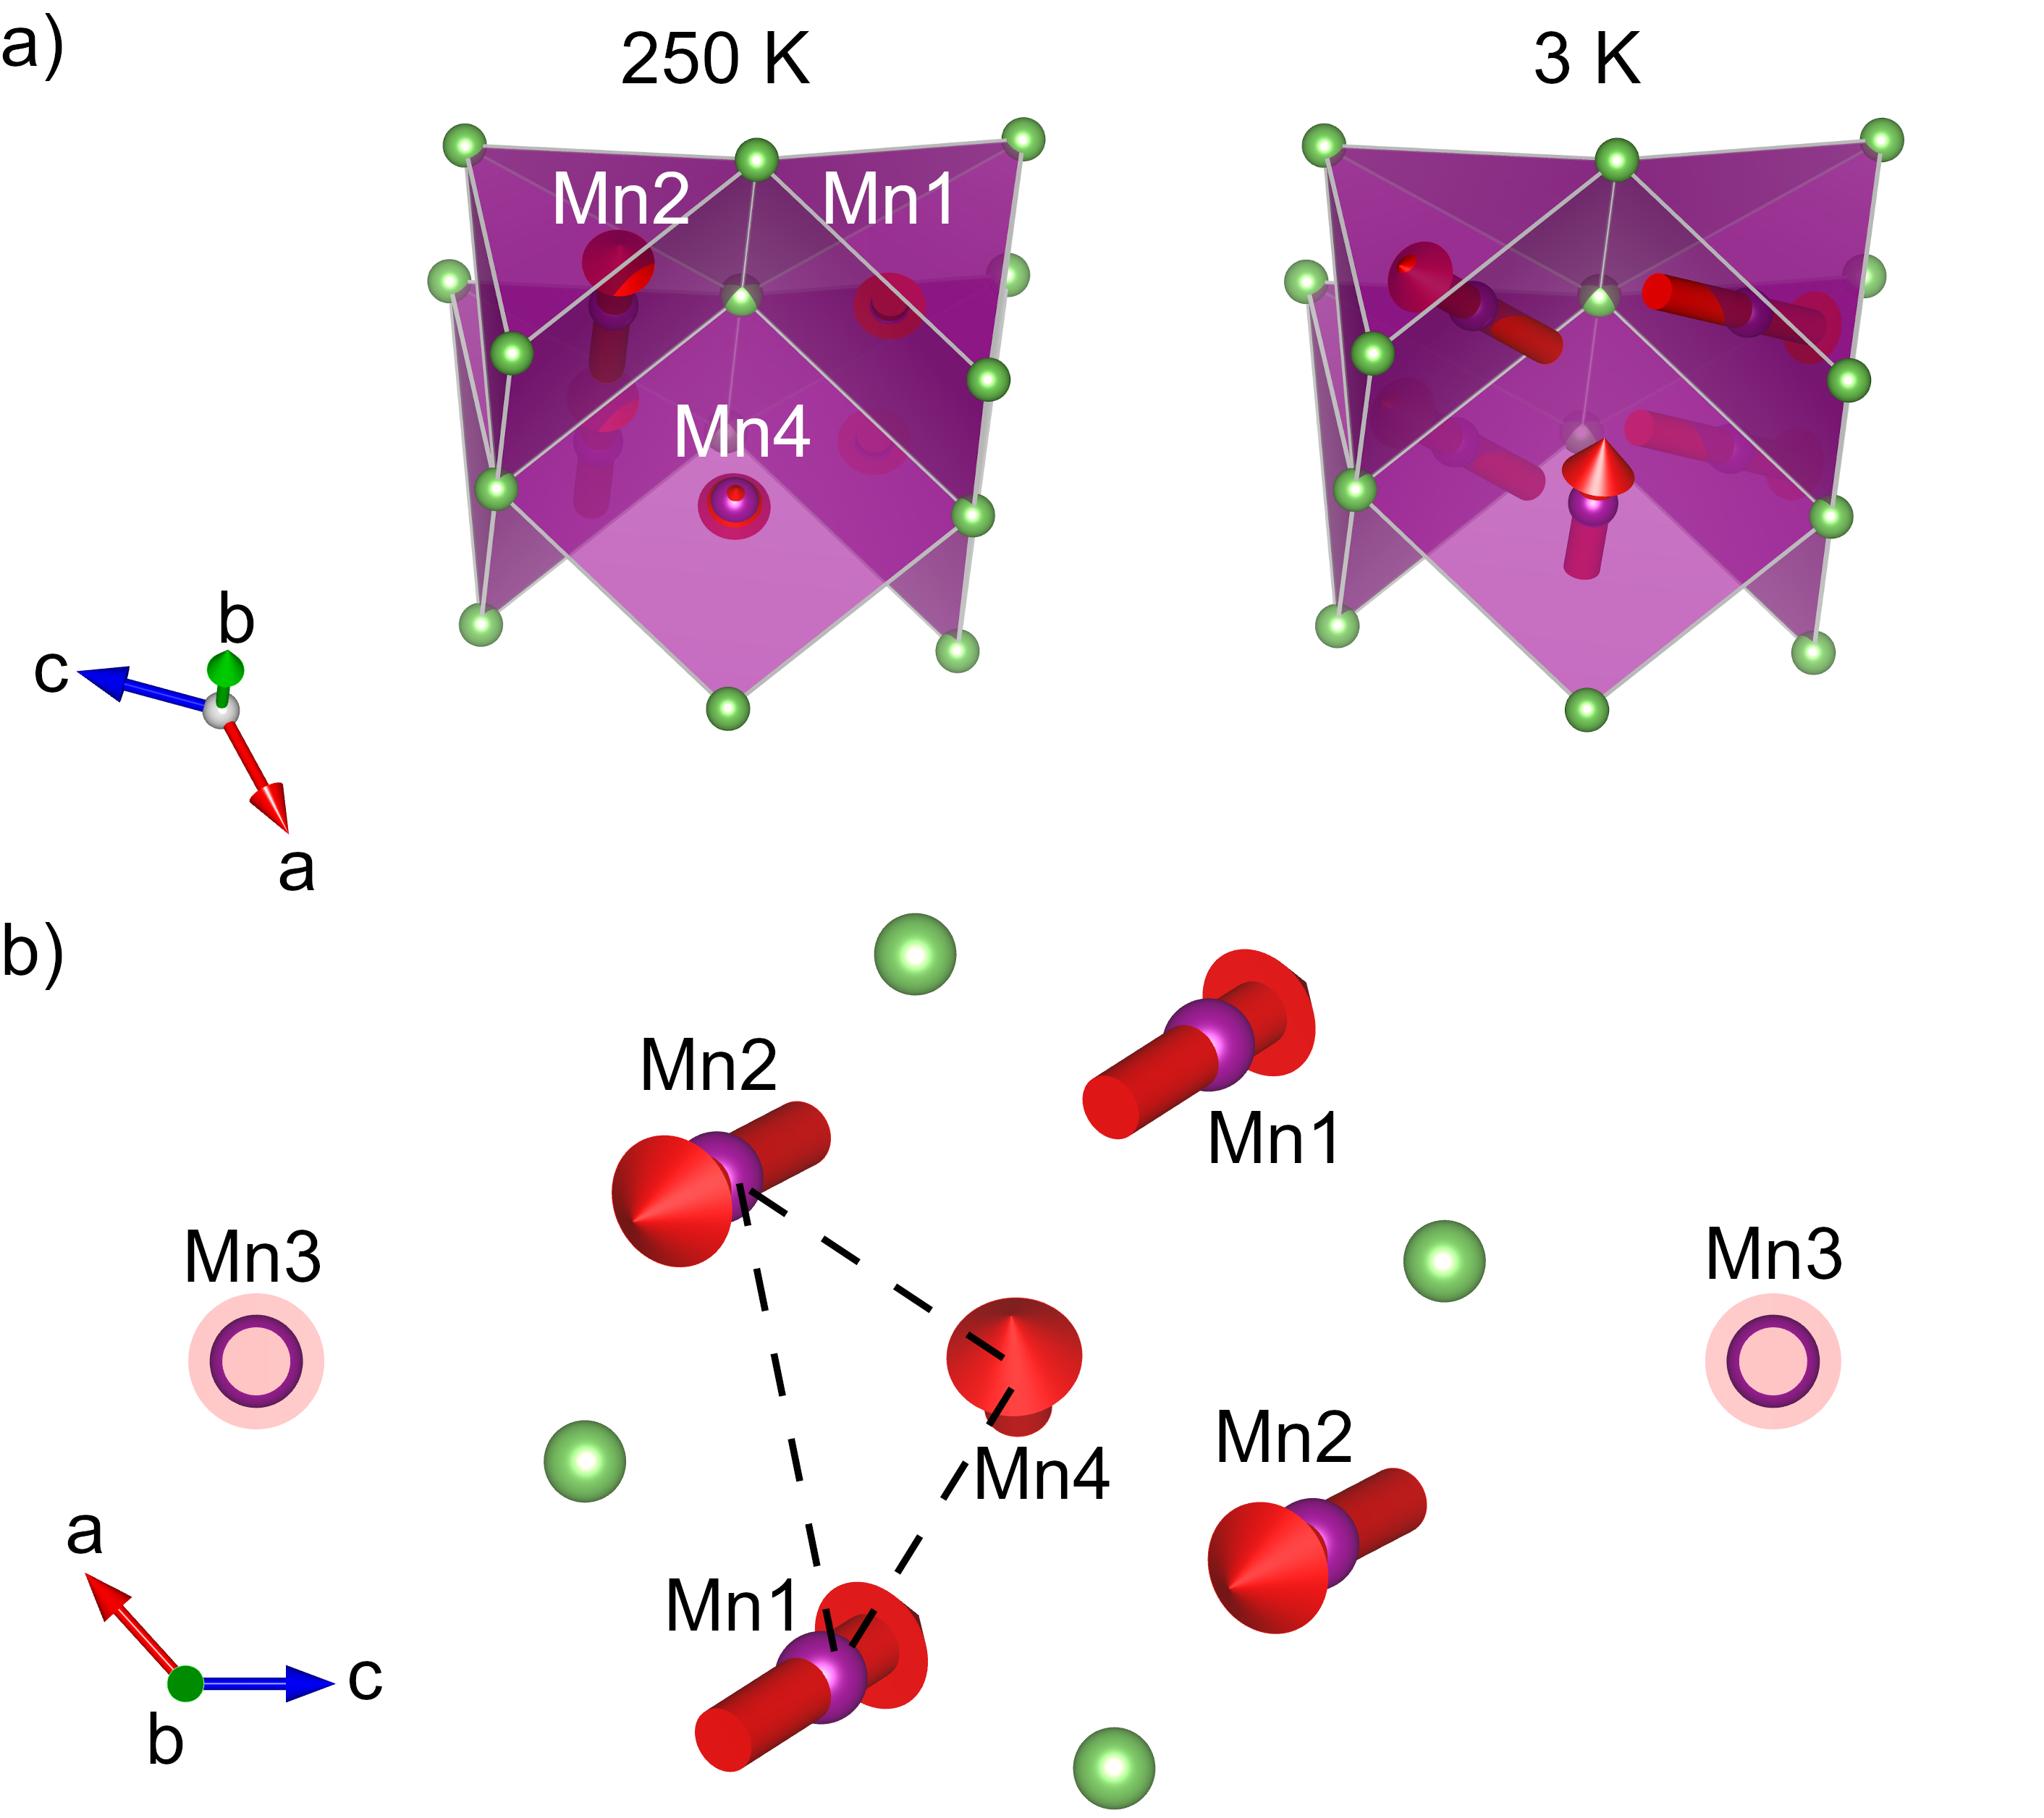
\includegraphics[width=\columnwidth]{figures/ch6/spin_canting_dps.png} \\
\caption{\label{fig:spin_canting}
Electronic band structure
}
\end{figure}

\begin{figure}
\centering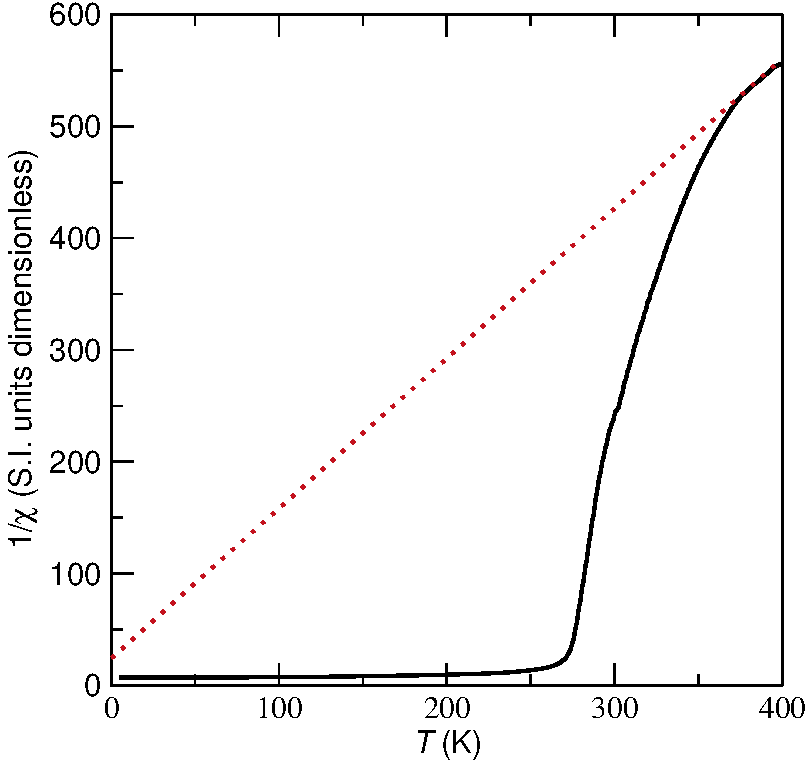
\includegraphics[width=\columnwidth]{figures/ch6/FC_52A_inverse_cropped.pdf} \\
\caption{\label{fig:inv_susceptibility}
Electronic band structure
}
\end{figure}

\Blindtext[6]

%chapter 7
\chapter{Spin canting in tetragonal CuMnAs}

\Blindtext[6]

%chapter 8
\chapter{Exchange interactions in Fe$_2$As probed by inelastic neutron scattering}

\begin{figure}
\centering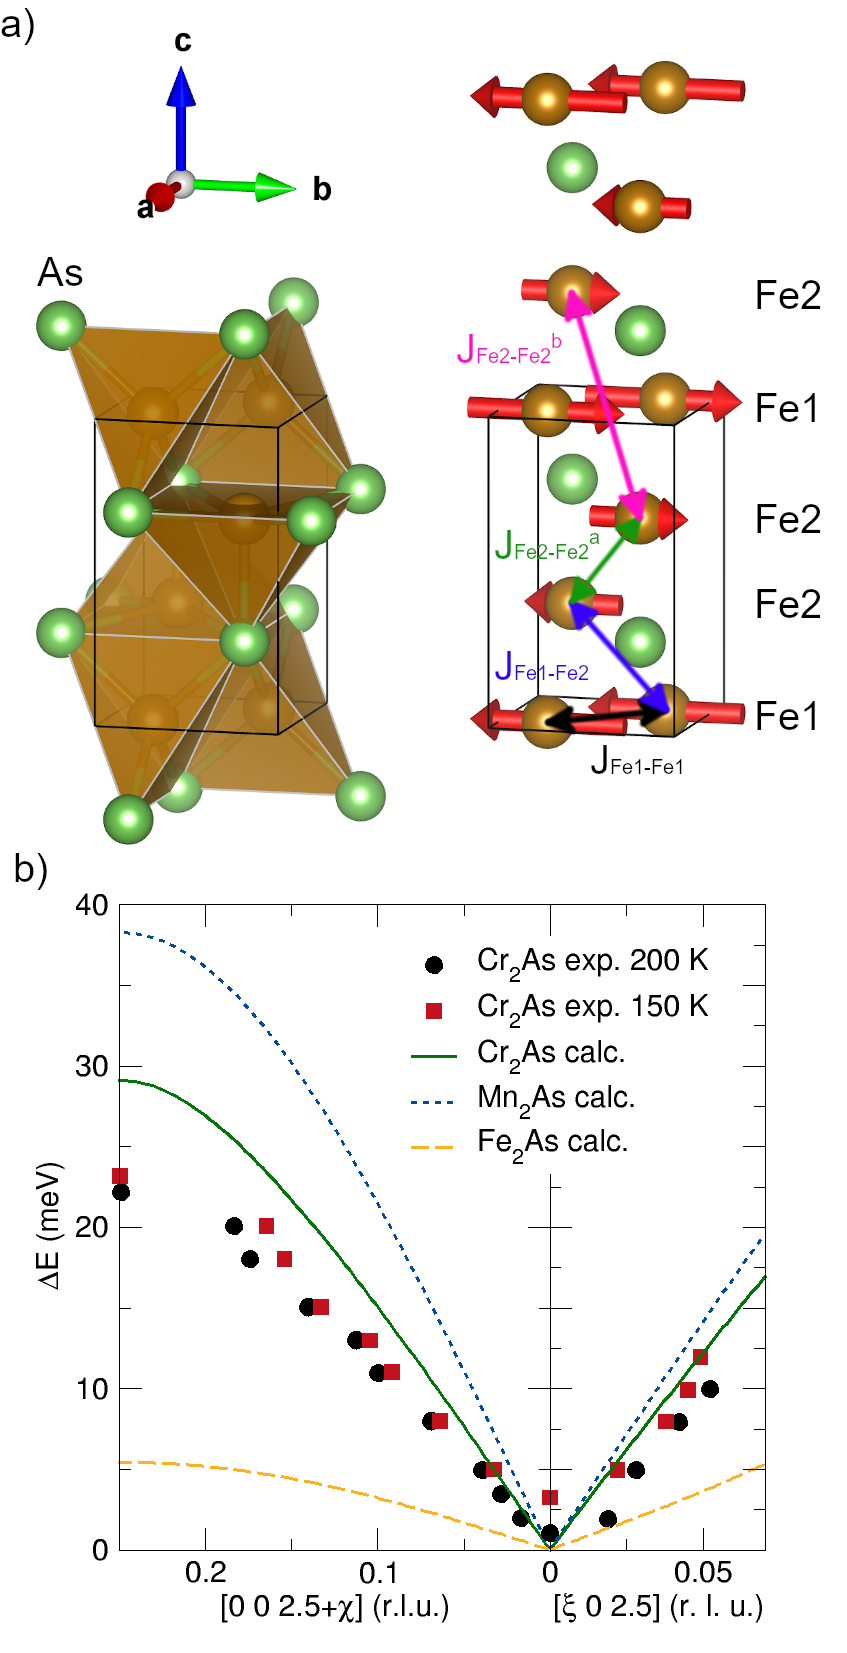
\includegraphics[width=0.5\columnwidth]{figures/ch8/Cr2As_INS_magnetic_structure.png} \\
\caption{\label{fig:Cr2As}
Electronic band structure
}
\end{figure}

\begin{figure}
\centering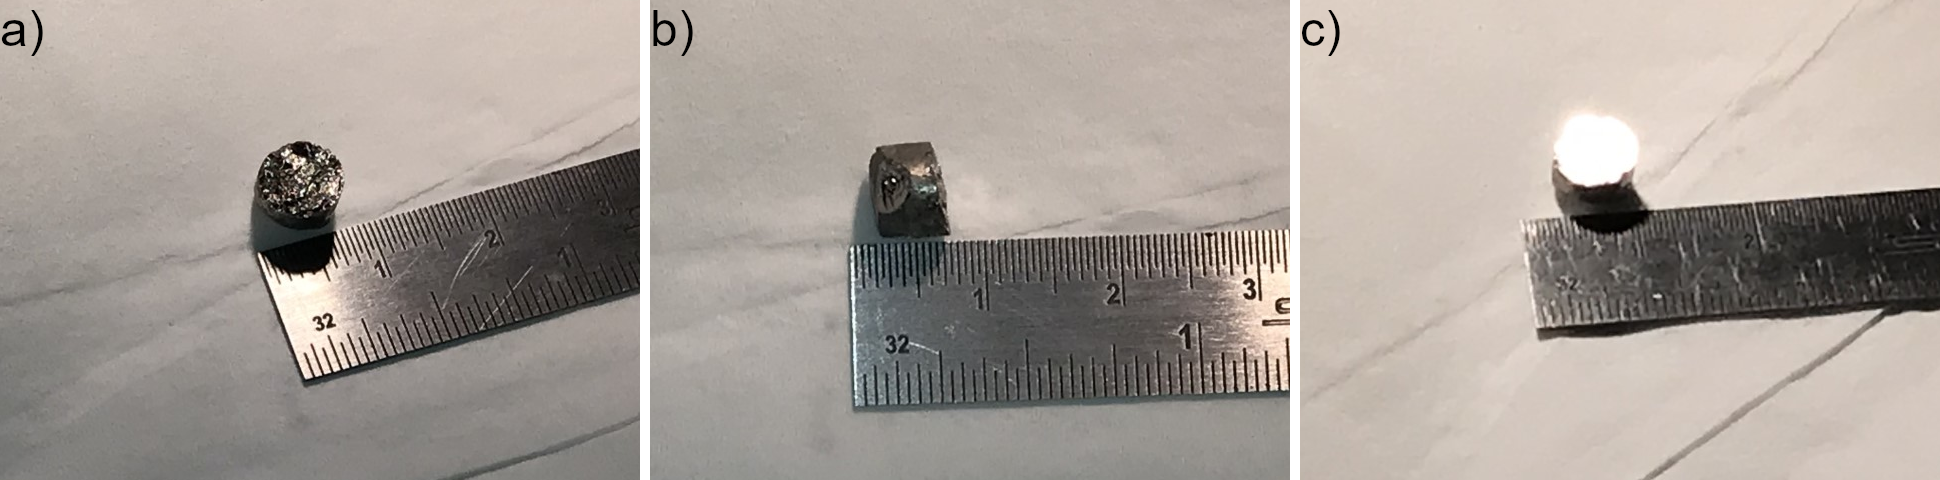
\includegraphics[width=\columnwidth]{figures/ch8/crystal.png} \\
\caption{\label{fig:crystal}
Electronic band structure
}
\end{figure}

\begin{figure}
\centering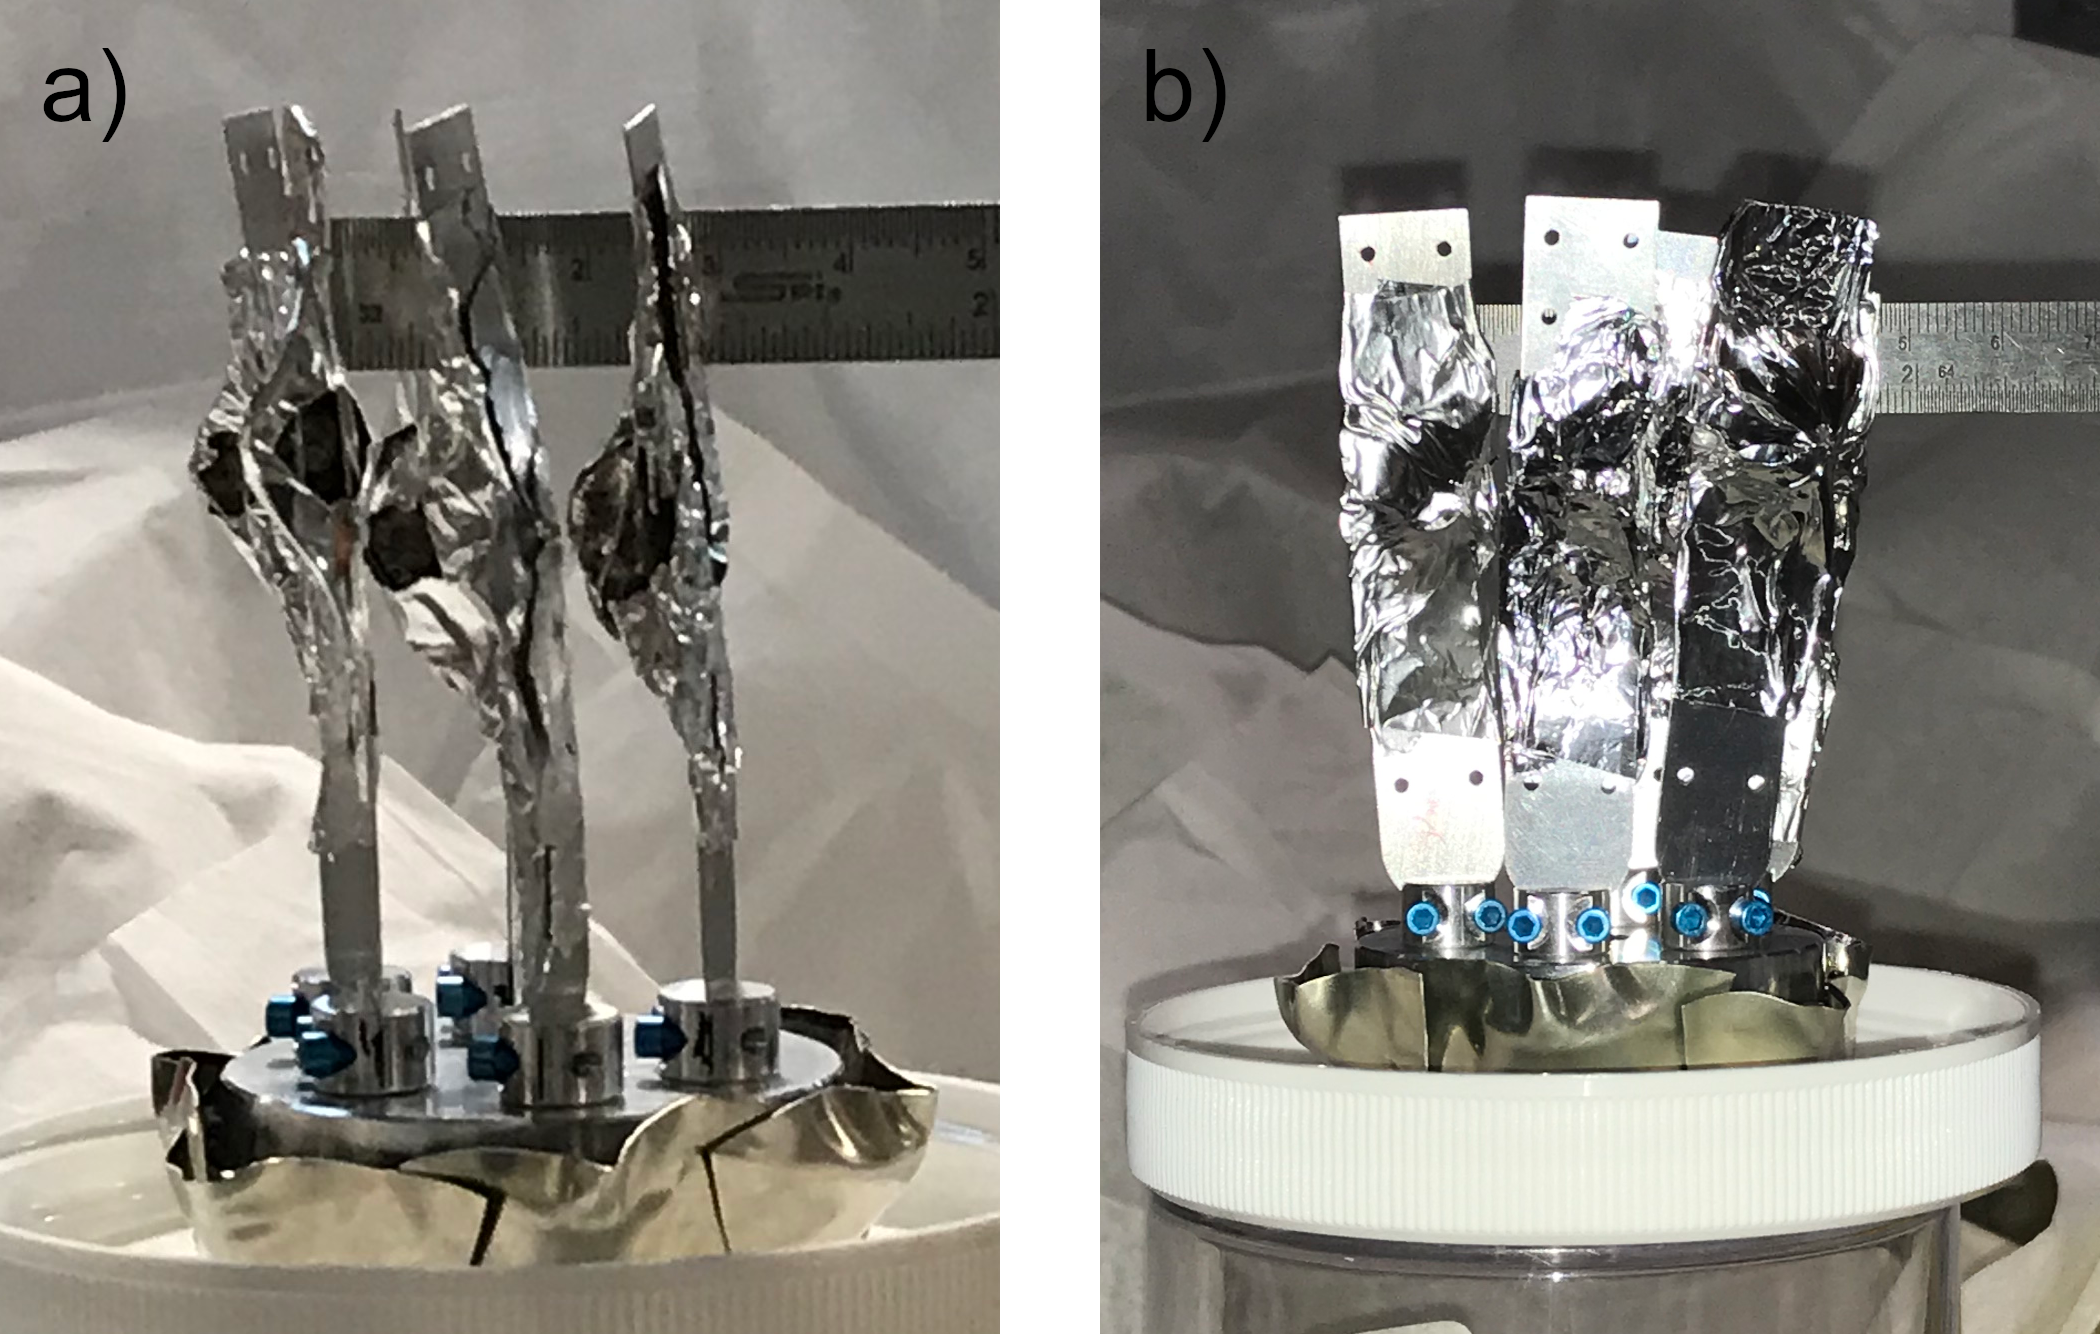
\includegraphics[width=\columnwidth]{figures/ch8/crystal_array.png} \\
\caption{\label{fig:crystal_array}
Electronic band structure
}
\end{figure}

\begin{figure}
\centering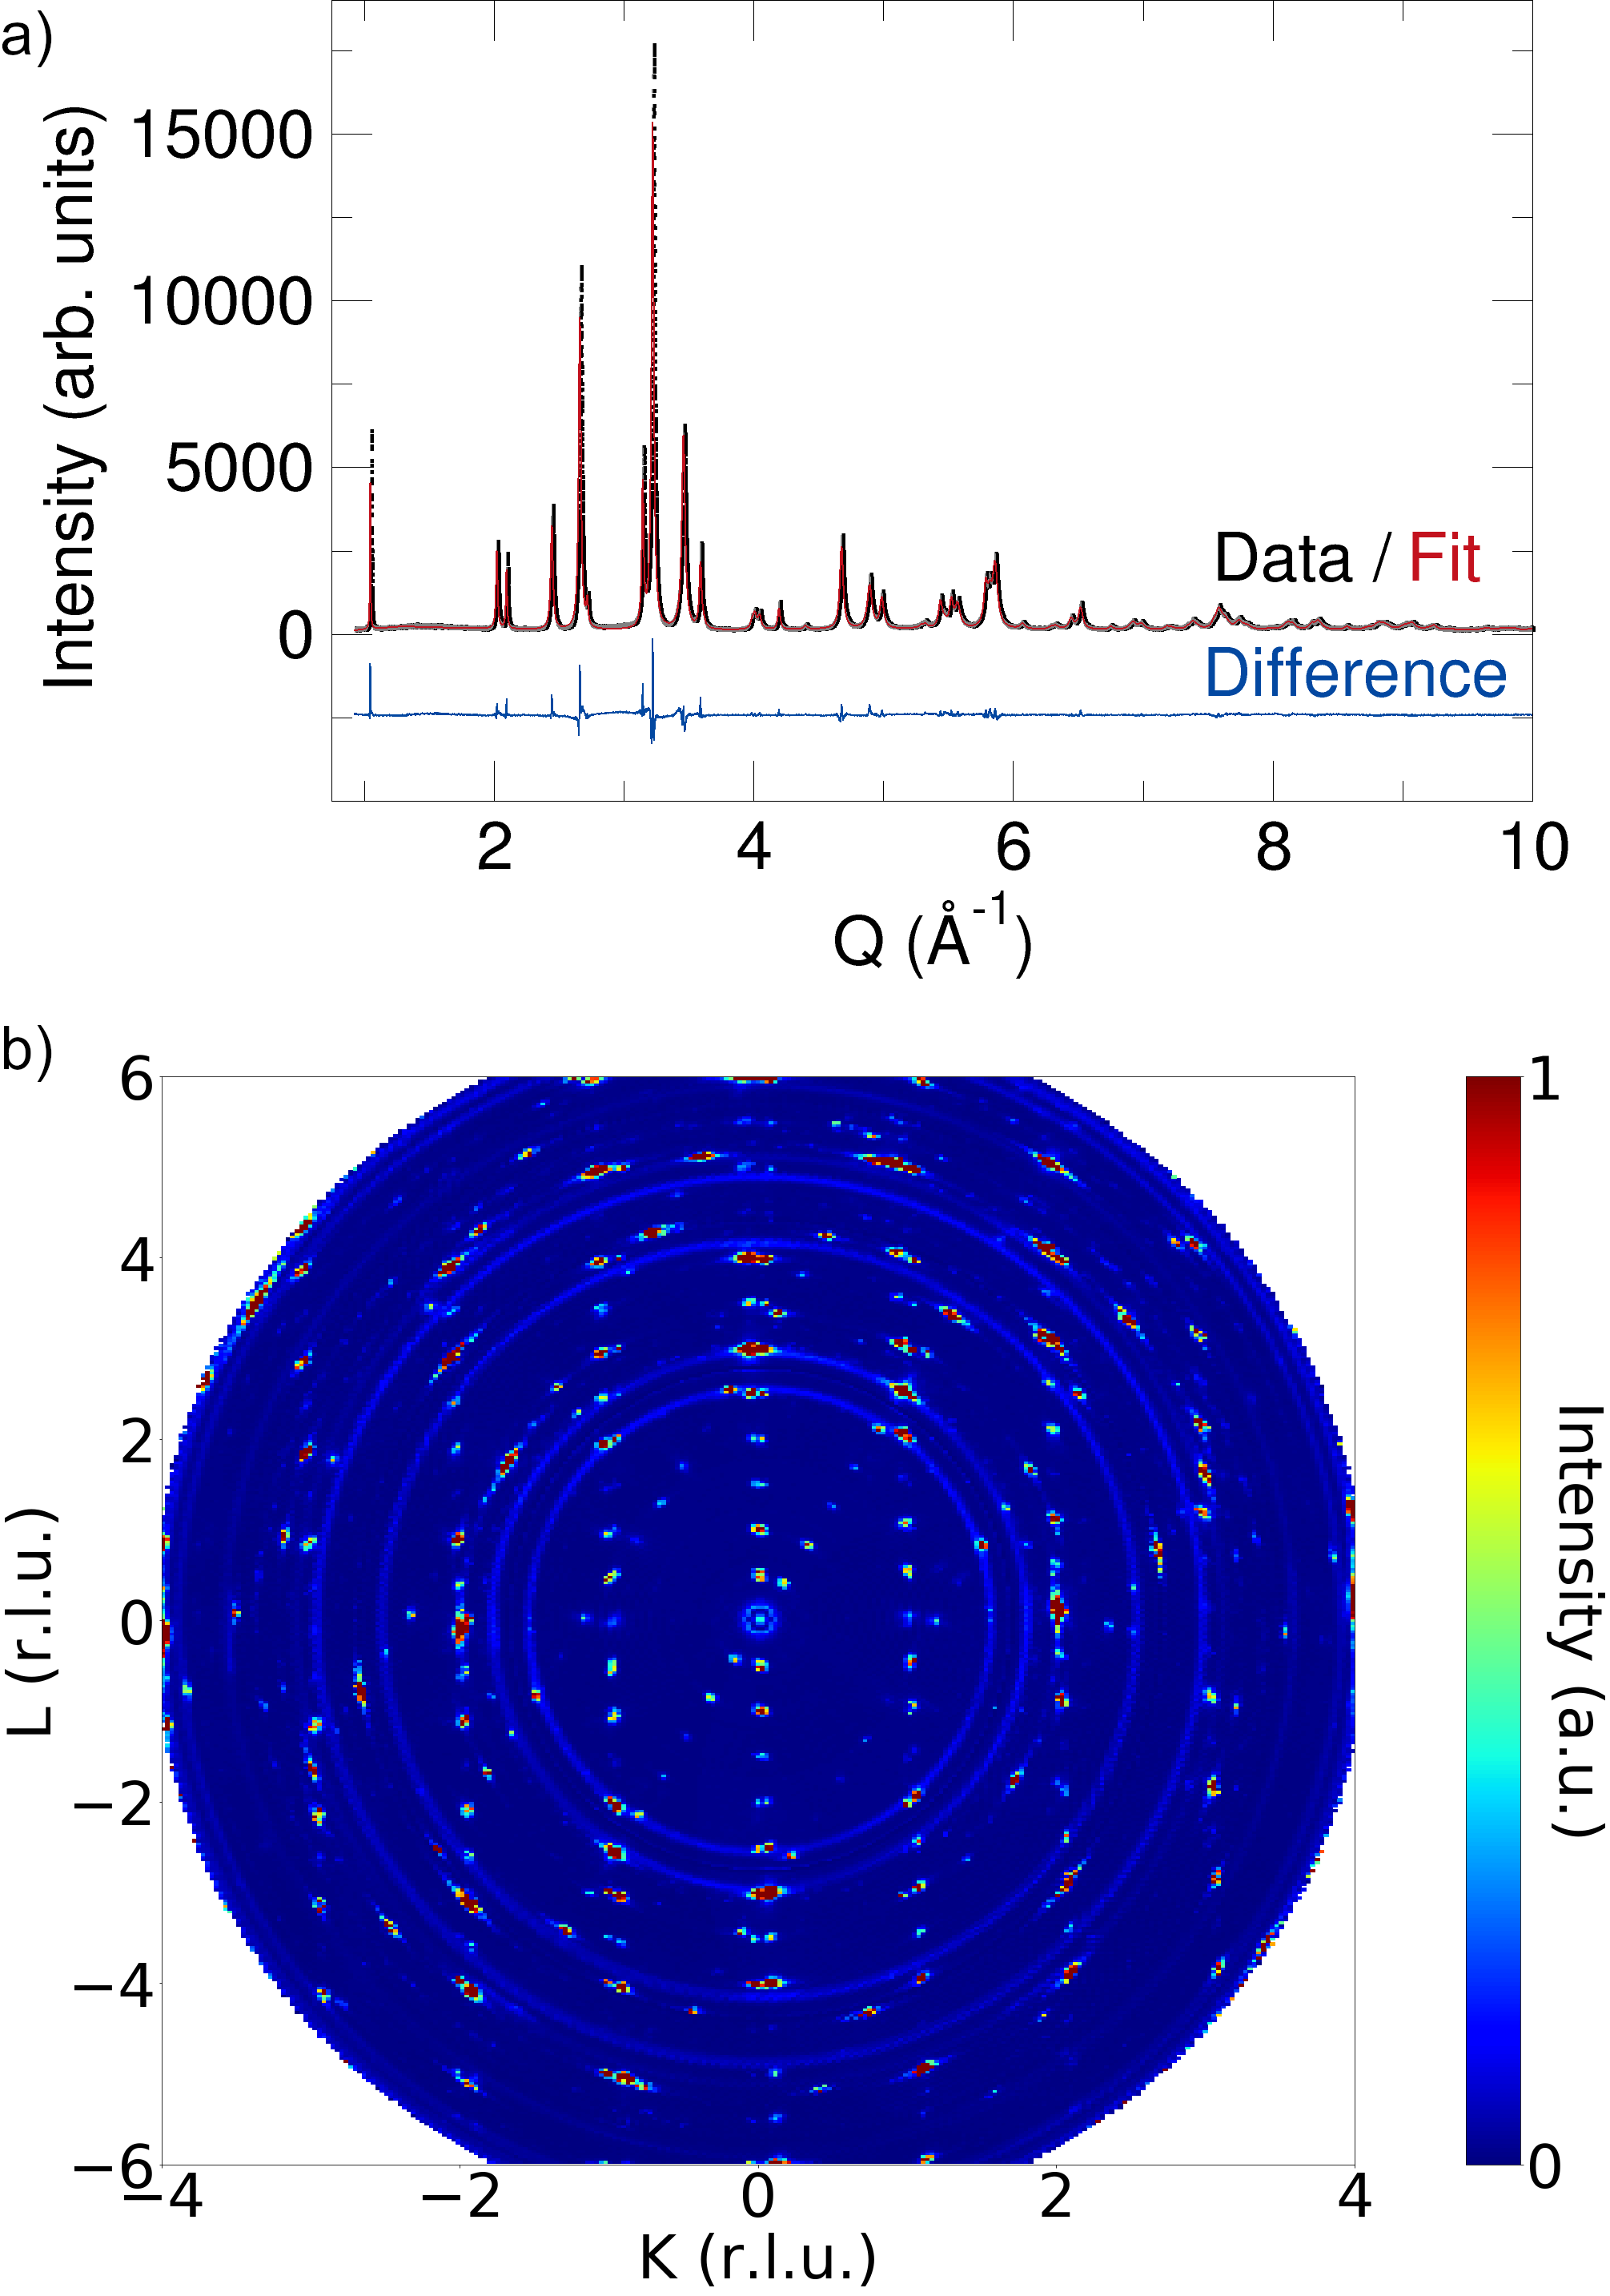
\includegraphics[width=\columnwidth]{figures/ch8/11BM_refinement_elastic_slice.png} \\
\caption{\label{fig:11BM_elastic_slice}
Electronic band structure
}
\end{figure}

\begin{figure}
\centering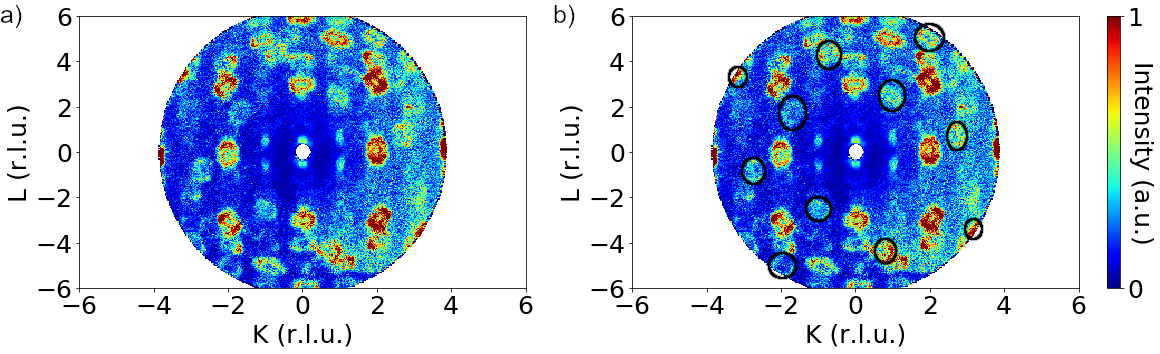
\includegraphics[width=0.7\columnwidth]{figures/ch8/suppl_misaligned_crystal_kl_slice.png} \\
\caption{\label{fig:misalign_crystal}
Electronic band structure
}
\end{figure}

\begin{figure}
\centering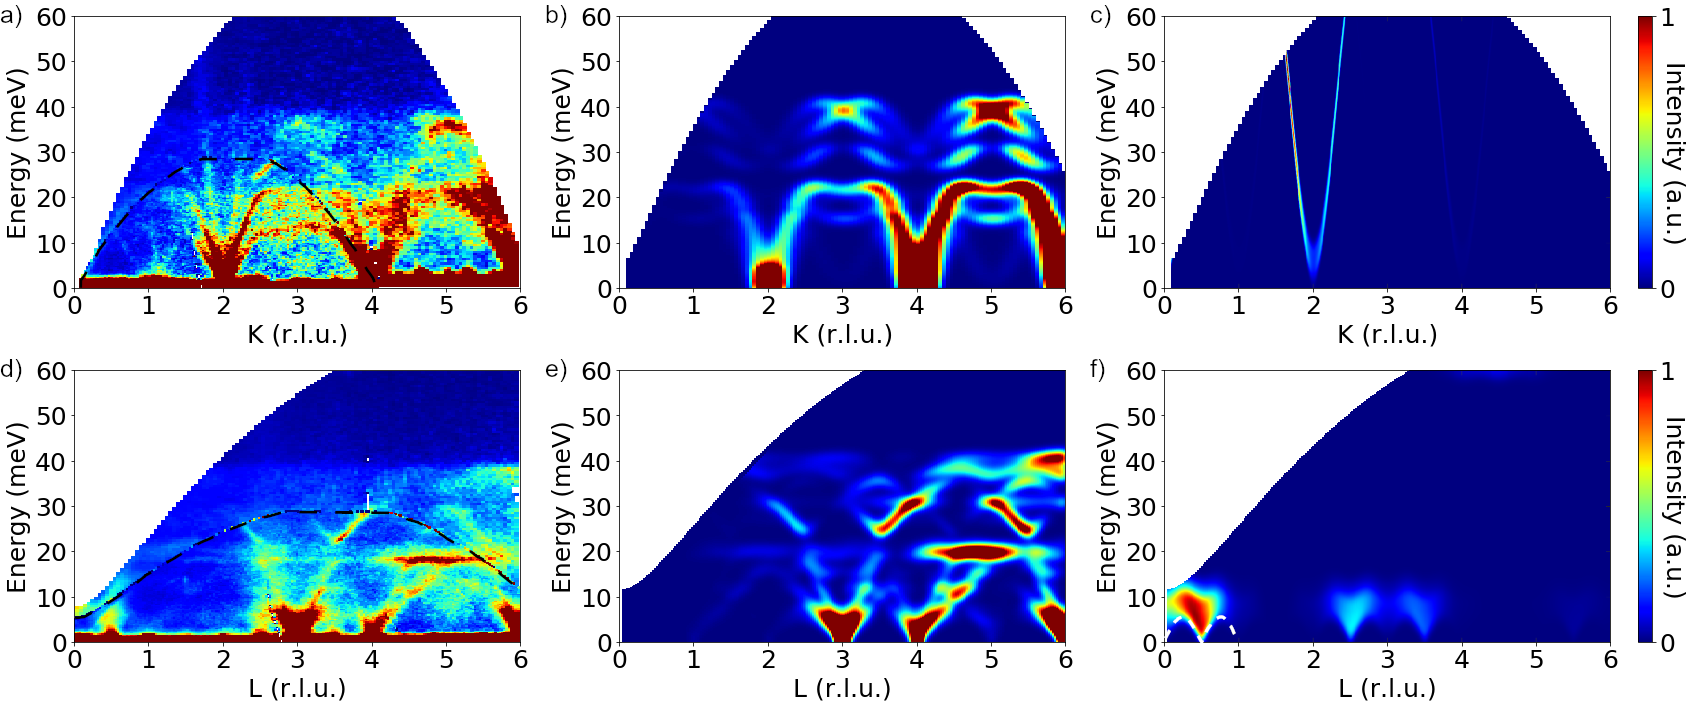
\includegraphics[width=\columnwidth]{figures/ch8/phonon_spectra_magnon_spectra_combined.png} \\
\caption{\label{fig:phonon_magnon_spectra}
Electronic band structure
}
\end{figure}

\begin{figure}
\centering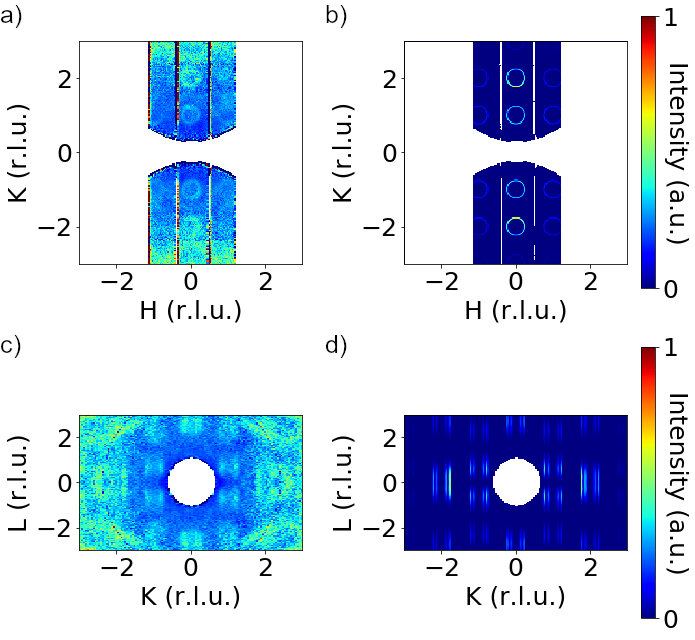
\includegraphics[width=\columnwidth]{figures/ch8/constant_energy_slices.png} \\
\caption{\label{fig:constant_energy_slices}
Electronic band structure
}
\end{figure}

\begin{figure}
\centering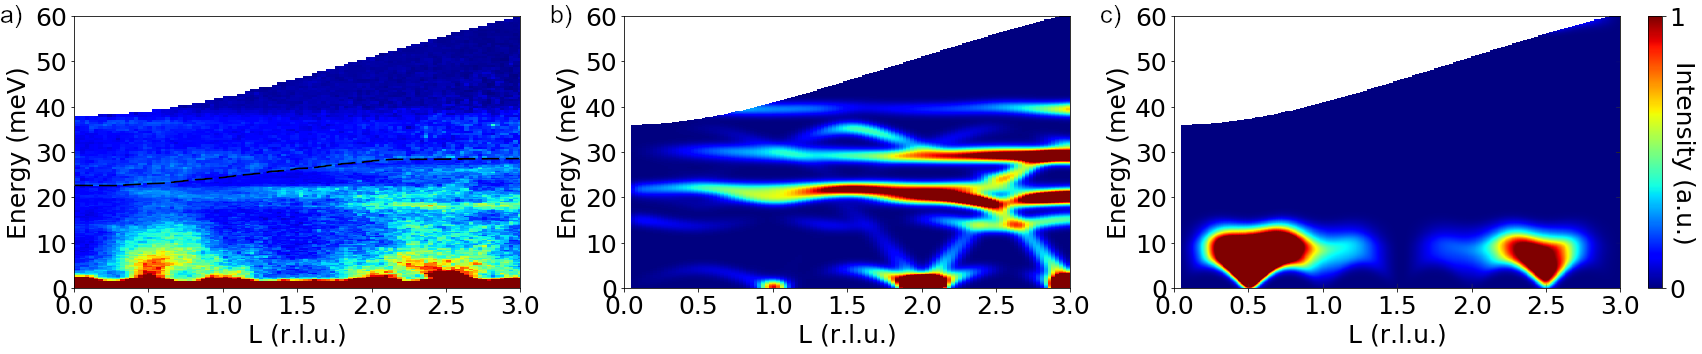
\includegraphics[width=\columnwidth]{figures/ch8/suppl_01L_INS_data.png} \\
\caption{\label{fig:01L_spectra}
Electronic band structure
}
\end{figure}

\begin{figure}
\centering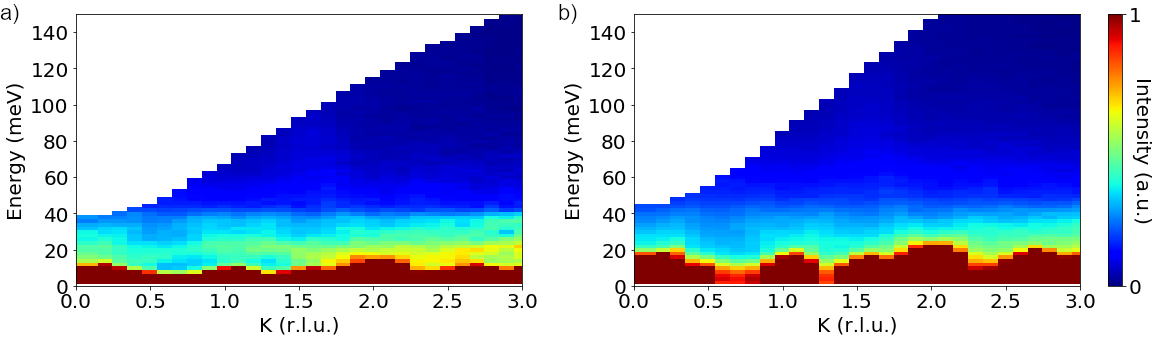
\includegraphics[width=\columnwidth]{figures/ch8/suppl_high_energy_data.png} \\
\caption{\label{fig:high_energy_data}
Electronic band structure
}
\end{figure}

\begin{figure}
\centering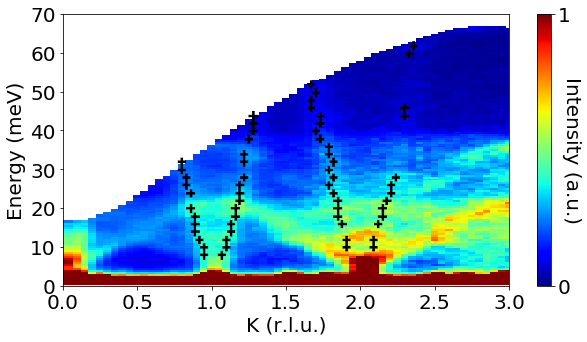
\includegraphics[width=\columnwidth]{figures/ch8/exp_data_points_0K0dot5.png} \\
\caption{\label{fig:exp_points}
Electronic band structure
}
\end{figure}

\begin{figure}
\centering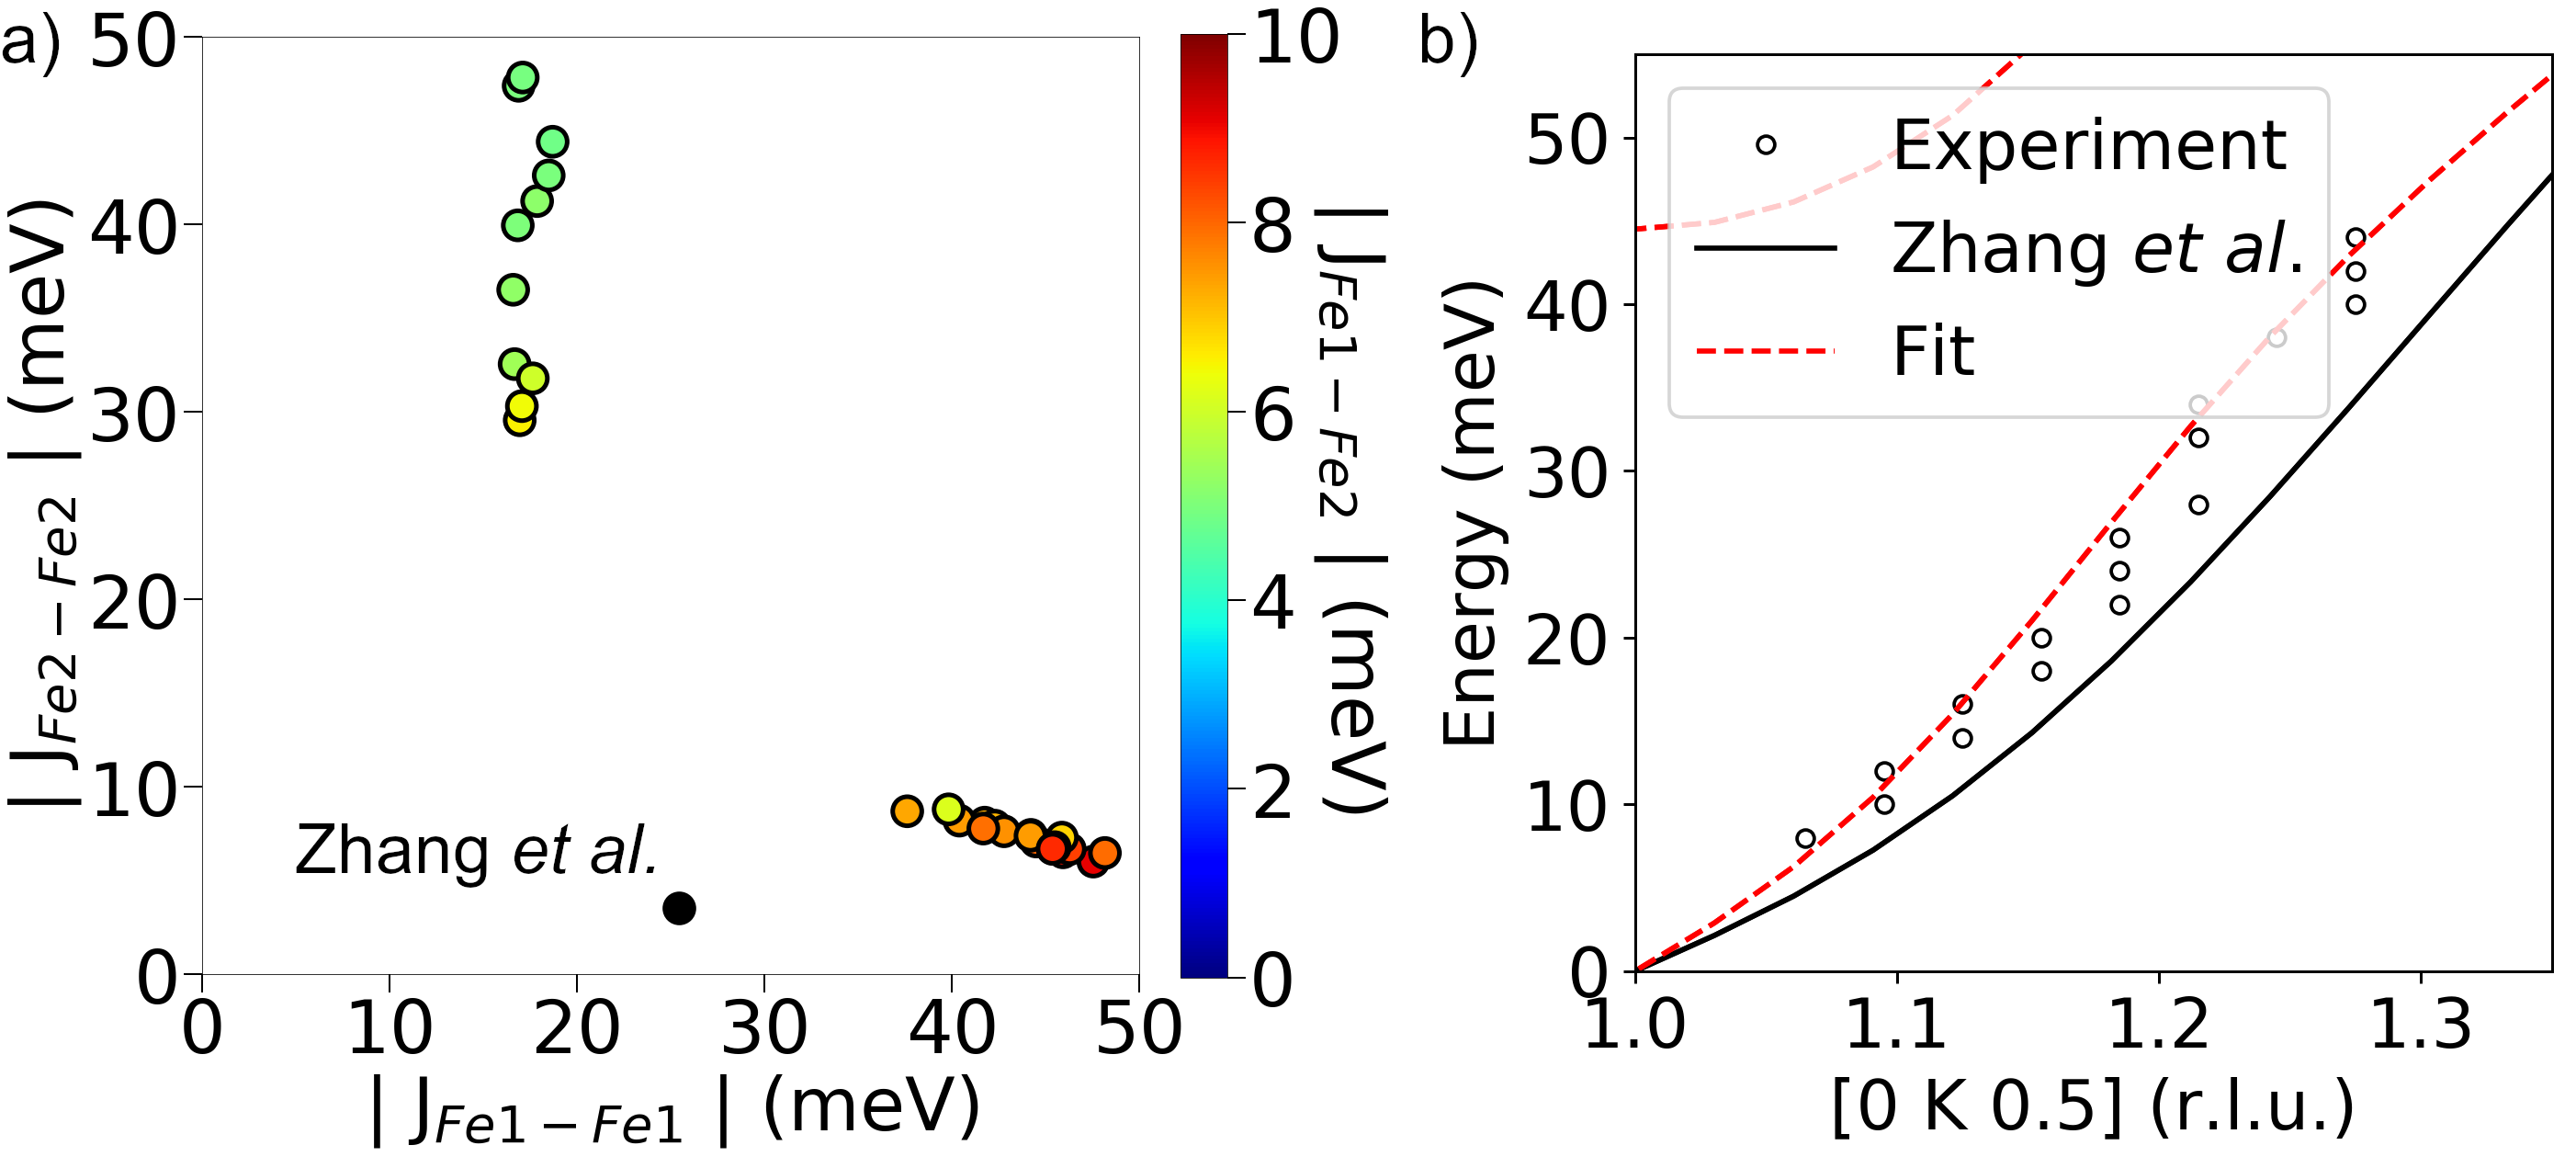
\includegraphics[width=\columnwidth]{figures/ch8/magnon_spectra_refinement.png} \\
\caption{\label{fig:refinement}
Electronic band structure
}
\end{figure}

\begin{figure}
\centering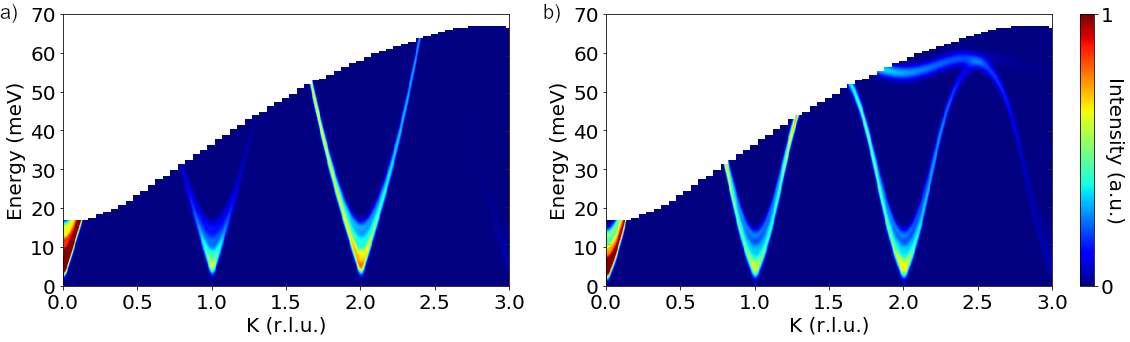
\includegraphics[width=\columnwidth]{figures/ch8/suppl_simulated_magnon_spectra_3J.png} \\
\caption{\label{fig:3J_fits}
Electronic band structure
}
\end{figure}

\Blindtext[6]

%chapter 9
\chapter{Conclusions}

\Blindtext[6]

\end{mainmatter}

% }}}

% {{{ back matter

\begin{backmatter}

\bibliographystyle{ieeetr}
\bibliography{thesis}

\end{backmatter}

%\appendix
%\chapter{My Appendix}

%\Blindtext[6]

% }}}

\end{document}
